\section{Descripción espacial y transformaciones}
\label{sec:descripcion_espacial}

La capacidad de definir la posición y orientación de objetos en el espacio tridimensional es esencial para controlar las extremidades y el cuerpo del robot. Para ello, se emplean sistemas de coordenadas y operaciones de álgebra lineal \cite{craig2018robotics,siciliano2016springer}.

\vspace{-0.5\baselineskip}
\subsection{Posición y orientación}

La posición de un punto en el espacio, expresada respecto a un sistema de referencia $\{A\}$, se describe mediante un vector de posición de dimensión $3\times1$. Sus componentes corresponden a las proyecciones ortogonales del punto sobre los ejes principales del sistema:

\vspace{-0.5\baselineskip}
\begin{equation}
    {}^A\bm{P} =
    \begin{bmatrix}
        {}^A P_x & {}^A P_y & {}^A P_z
    \end{bmatrix}^T
    \label{eq:vector_posicion}
\end{equation}
\vspace{-1.0\baselineskip}

Sin embargo, para definir unívocamente el estado de un cuerpo rígido en el espacio, la posición no es suficiente; es necesario especificar también su orientación. Para ello se emplea la \textbf{matriz de rotación}, cuyos vectores columna representan los vectores unitarios de los ejes del sistema rotado $\{B\}$ expresados en la base del sistema de referencia $\{A\}$:

\vspace{-0.5\baselineskip}
\begin{equation}
    {}^A\bm{R}_B = 
    \begin{bmatrix}
        {}^A\hat{X}_B & {}^A\hat{Y}_B & {}^A\hat{Z}_B
    \end{bmatrix}
    =
    \begin{bmatrix}
        \hat{X}_B \cdot \hat{X}_A & \hat{Y}_B \cdot \hat{X}_A & \hat{Z}_B \cdot \hat{X}_A \\
        \hat{X}_B \cdot \hat{Y}_A & \hat{Y}_B \cdot \hat{Y}_A & \hat{Z}_B \cdot \hat{Y}_A \\
        \hat{X}_B \cdot \hat{Z}_A & \hat{Y}_B \cdot \hat{Z}_A & \hat{Z}_B \cdot \hat{Z}_A
    \end{bmatrix}
    \label{eq:rij_productos_escalares}
\end{equation}
\vspace{-0.5\baselineskip}

Dado que ${}^A\bm{R}_B$ contiene nueve elementos pero solo tres grados de libertad, resulta conveniente parametrizarla mediante tres ángulos. En este TFG se adopta la convención de ángulos fijos $X$-$Y$-$Z$ (\textit{roll-pitch-yaw}) de la Figura~\ref{fig:rpy_axes}, que compone las rotaciones elementales en orden inverso ($Z \rightarrow Y \rightarrow X$) \cite{craig2018robotics}:


\begin{figure}[H]
    \vspace{-0.5\baselineskip}
    \centering
    \begin{minipage}[c]{0.40\textwidth}
        \begin{equation}
            {}^A\bm{R}_B = R_z(\alpha)\,R_y(\beta)\,R_x(\gamma)
            \label{eq:Rypr_comp}
        \end{equation}
    \end{minipage}%
    \hfill
    \begin{minipage}[c]{0.60\textwidth}
        \centering
        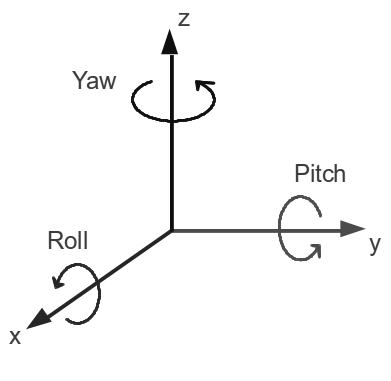
\includegraphics[width=0.50\linewidth]{capitulos/cap2/figuras/rpy_axes.png}
    \end{minipage}
    \captionsetup{justification=centering}
    \caption[Ejes de roll, pitch y yaw]{Ejes de rotación roll, pitch y yaw sobre un cuerpo rígido.}
    \label{fig:rpy_axes}
    {\footnotesize Fuente: adaptado de Aldebaran Robotics \cite{aldebaran_rpy_axes}.}
    \vspace{-0.5\baselineskip}
\end{figure}

En la Ec.~\ref{eq:Rypr_comp}, $\alpha$, $\beta$ y $\gamma$ son los ángulos de \textit{yaw}, \textit{pitch} y \textit{roll}, es decir, los giros en torno a los ejes $Z$, $Y$ y $X$, respectivamente. Desarrollando cada rotación elemental, la matriz resulta:

\begin{equation}
    {}^A\bm{R}_B
    =
    \underbrace{
    \begin{bmatrix}
        \cos\alpha & -\sin\alpha & 0 \\
        \sin\alpha & \cos\alpha  & 0 \\
        0          & 0           & 1
    \end{bmatrix}}_{R_z(\alpha)}
    \underbrace{
    \begin{bmatrix}
        \cos\beta & 0 & \sin\beta \\
        0         & 1 & 0 \\
        -\sin\beta& 0 & \cos\beta
    \end{bmatrix}}_{R_y(\beta)}
    \underbrace{
    \begin{bmatrix}
        1 & 0          & 0 \\
        0 & \cos\gamma & -\sin\gamma \\
        0 & \sin\gamma & \cos\gamma
    \end{bmatrix}}_{R_x(\gamma)}
    \label{eq:Rzyx_producto_elementales}
\end{equation}

\subsection{Definición de sistema de coordenadas y transformaciones}

La combinación de posición y orientación permite definir el concepto de sistema de coordenadas, la entidad fundamental en robótica para describir la ubicación de un eslabón o cuerpo. Geométricamente, un sistema de coordenadas $\{B\}$ queda completamente definido respecto a $\{A\}$ mediante el par ordenado:

\vspace{-0.5\baselineskip}
\begin{equation}
    \{B\}\ \text{respecto a}\ \{A\}
    \ \equiv\
    \left( {}^A\bm{R}_B,\ {}^A\bm{P}_B \right)
    \label{eq:def_frame_R_P}
\end{equation}
\vspace{-0.75\baselineskip}

donde ${}^A\bm{R}_B$ es la orientación de $\{B\}$ respecto a $\{A\}$ y ${}^A\bm{P}_B$ es el vector de posición del origen de $\{B\}$ expresado en $\{A\}$. Esta estructura permite transformar las coordenadas de cualquier punto $\bm{P}$ descrito en el sistema local $\{B\}$ al sistema de referencia global $\{A\}$ mediante la ecuación fundamental de transformación de cuerpo rígido (Figura~\ref{fig:def_frame_transform}):

\vspace{-0.5\baselineskip}
\begin{figure}[H]
    \centering
    % --- CAJA IZQUIERDA: La Ecuación (40% del ancho) ---
    \begin{minipage}[c]{0.40\textwidth}
        \begin{equation}
            {}^A\bm{P} = {}^A\bm{R}_B \, {}^B\bm{P} + {}^A\bm{P}_B
            \label{eq:transformacion_fundamental}
        \end{equation}
    \end{minipage}%
    \hfill % Relleno flexible para separarlas
    % --- CAJA DERECHA: La Imagen (55% del ancho) ---
    \begin{minipage}[c]{0.55\textwidth}
        \centering
        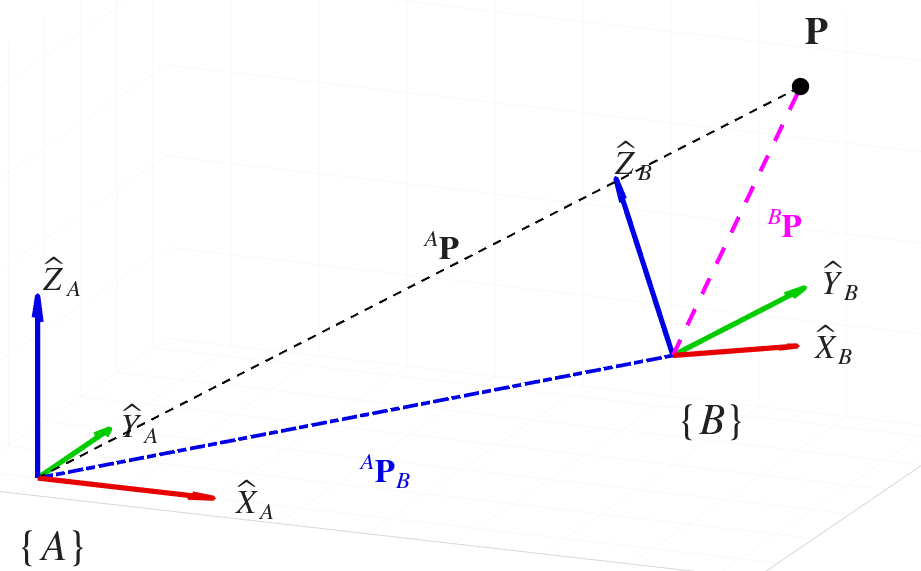
\includegraphics[width=\linewidth]{capitulos/cap2/figuras/composicionframes.png}
    \end{minipage}

    % Pie de figura para todo el conjunto
    \caption[Representación geométrica de un sistema de coordenadas]{Relación espacial entre dos sistemas de coordenadas. La ecuación describe la transformación del punto $P$ del sistema $\{B\}$ al sistema global $\{A\}$.}
    \label{fig:def_frame_transform}
    {\footnotesize Fuente: Elaboración propia mediante MATLAB~\cite{matlab}.}
\end{figure}
\vspace{-0.5\baselineskip}

Esto se puede expresar de forma más compacta mediante el uso de la matriz de transformación homogénea que describe el sistema $\{B\}$ respecto a $\{A\}$ \cite{craig2018robotics,siciliano2016springer} como:

\vspace{-0.5\baselineskip}
\begin{equation}
    {}^A\mathbf{T}_B = 
    \begin{bmatrix} 
        {}^A\bm{R}_B & {}^A\bm{P}_B\\ 
        \bm{0}_{1\times 3} & 1 
    \end{bmatrix}
    \label{eq:T_homogenea}
\end{equation}

De esta forma, la transformación fundamental de la Ec.~\ref{eq:transformacion_fundamental} se escribe en forma homogénea como:

\vspace{-0.5\baselineskip}
\begin{equation}
    {}^A\tilde{\bm{P}} = {}^A\mathbf{T}_B \; {}^B\tilde{\bm{P}}
    \label{eq:transformacion_homogenea}
\end{equation}

donde los vectores de posición se expresan en coordenadas homogéneas de dimensión $4\times1$, añadiendo una cuarta componente unitaria ($\tilde{\bm{P}} = [\bm{P}^T\ \ 1]^T$). De esta forma, al desarrollar la Ec.~\ref{eq:transformacion_homogenea} se recupera directamente la expresión en $\mathbb{R}^3$:

\vspace{-0.5\baselineskip}
\begin{equation}
    {}^A\tilde{\bm{P}}
    =
    \begin{bmatrix}
        {}^A\bm{P}\\
        1
    \end{bmatrix}
    =
    \begin{bmatrix}
        {}^A\bm{R}_B\,{}^B\bm{P} + {}^A\bm{P}_B\\
        1
    \end{bmatrix}
\end{equation}

\subsubsection{Propiedades algebraicas}

La ventaja principal de esta representación es la capacidad de \textbf{concatenar} transformaciones relativas mediante multiplicación matricial \cite{craig2018robotics,siciliano2016springer}. Si se conocen ${}^A\mathbf{T}_B$ y ${}^B\mathbf{T}_C$, entonces:

\vspace{-0.5\baselineskip}
\begin{equation}
    {}^A\mathbf{T}_C = {}^A\mathbf{T}_B \; {}^B\mathbf{T}_C=\begin{bmatrix}
        {}^A\bm{R}_B\,{}^B\bm{R}_C &
        {}^A\bm{R}_B\,{}^B\bm{P}_C + {}^A\bm{P}_B\\
        \bm{0}_{1\times 3} & 1
    \end{bmatrix}
    \label{eq:concatenacion_T}
\end{equation}

Es importante observar que la traslación de la segunda transformación, ${}^B\bm{P}_C$, está expresada en $\{B\}$, por lo que debe rotarse mediante ${}^A\bm{R}_B$ para expresarla en $\{A\}$ antes de sumarle ${}^A\bm{P}_B$, tal y como se ilustra en la Figura~\ref{fig:concatenacion_frames}.

% --- FIGURA 2: CONCATENACIÓN ---
\begin{figure}[H]
    \centering
    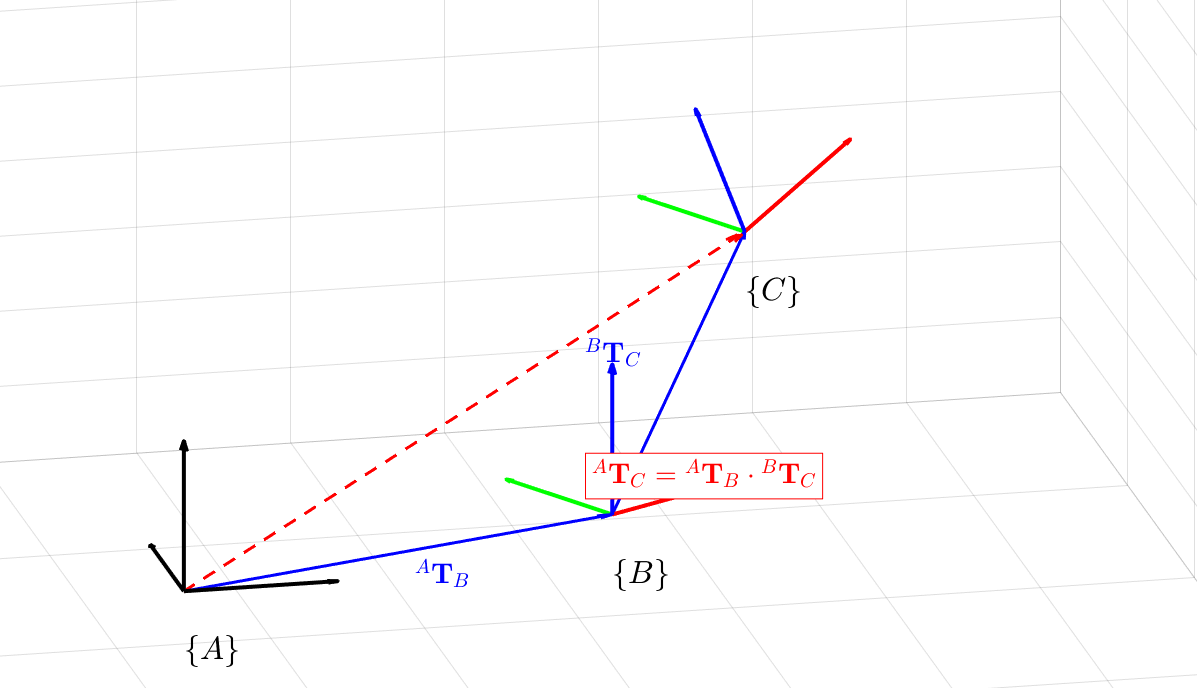
\includegraphics[width=0.6\textwidth]{capitulos/cap2/figuras/concatenacion.png}
    \caption[Concatenación de transformaciones]{Concatenación de transformaciones espaciales. La transformación global ${}^A\mathbf{T}_C$ puede obtenerse mediante la composición de las transformaciones intermedias.}
    \label{fig:concatenacion_frames}
    {\footnotesize Fuente: Elaboración propia.}
\end{figure}
\vspace{-0.5\baselineskip}

Esto es esencial en robótica, donde es habitual encadenar sistemas de coordenadas para obtener la posición final. También es frecuente transformar en sentido contrario (por ejemplo, de $\{A\}$ a $\{B\}$). La inversa de una transformación homogénea tiene forma cerrada:

\begin{equation}
    ({}^A\mathbf{T}_B)^{-1} = {}^B\mathbf{T}_A = 
    \begin{bmatrix} 
        ({}^A\bm{R}_B)^T & -({}^A\bm{R}_B)^T\,{}^A\bm{P}_B\\ 
        \bm{0} & 1 
    \end{bmatrix}
    \label{eq:T_inversa}
\end{equation}

donde se ha utilizado la propiedad de ortogonalidad de las matrices de rotación:
\begin{equation}
    ({}^A\bm{R}_B)^{-1} = ({}^A\bm{R}_B)^T
    \label{eq:R_inv_RT}
\end{equation}

Esta propiedad simplifica la implementación: para invertir una rotación basta con trasponer la matriz, sin necesidad de inversión numérica, lo que reduce la carga computacional en cada iteración de control.


\section{Cinemática directa del cuerpo}
\label{sec:cinematica_cuerpo}

En un hexápodo controlado mediante posiciones de extremo (\textit{endpoints}), la postura del cuerpo fija de forma directa la posición relativa de las patas y, por tanto, los objetivos cartesianos que cada una debe alcanzar. Por ello, la cinemática del cuerpo debe formularse de manera coherente con la cinemática de las patas, lo que exige modelar la posición del chasis respecto al sistema global y describir su evolución temporal.

\subsection{Sistemas de coordenadas y notación}
\label{subsec:frames_notacion}

Se emplean tres sistemas de referencia principales:

\begin{figure}[H]
    \centering

    \begin{minipage}{0.95\textwidth}
        \begin{itemize}
            \item $\{G\}$: sistema global (GLOBAL), fijo al terreno, alineado verticalmente
            \item $\{B\}$: sistema del cuerpo (BODY), solidario al chasis.
            \item $\{L_i\}$: sistema local de la pata $i$ (LEG), ubicado en la articulación de la coxa, el comienzo de la extremidad.
        \end{itemize}
    \end{minipage}


    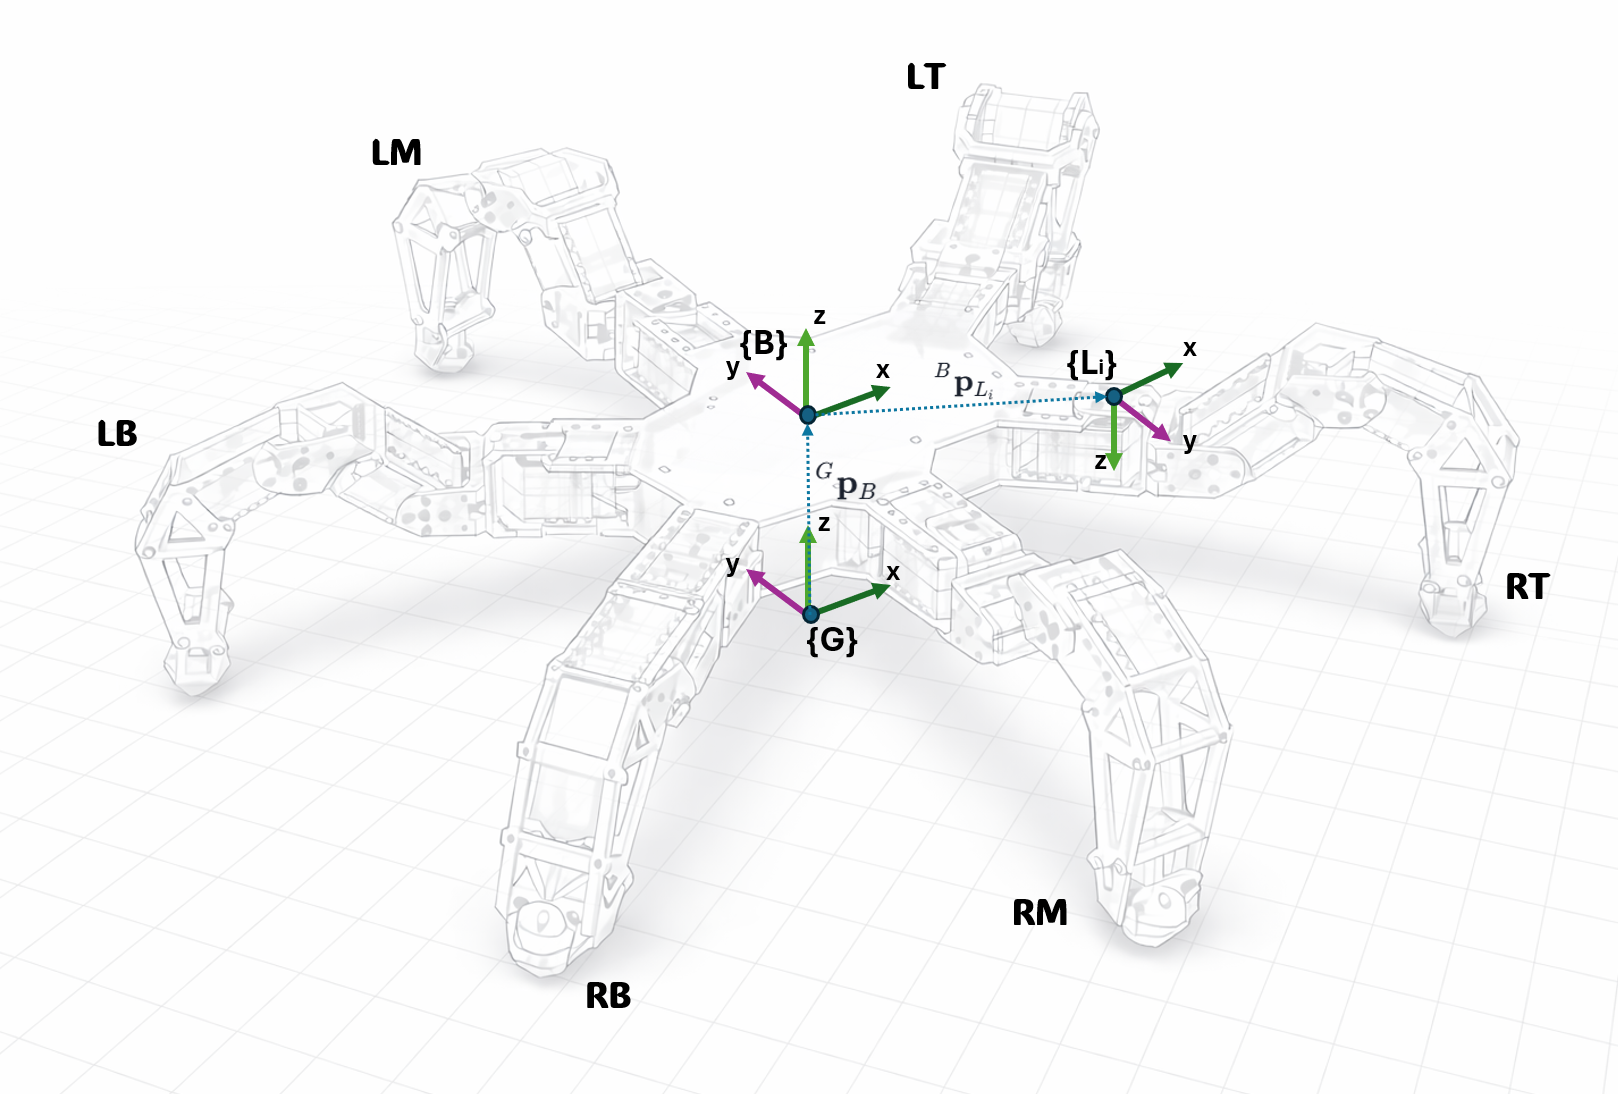
\includegraphics[width=1.00\textwidth]{capitulos/cap2/figuras/frames.png}

    \captionsetup{justification=centering}
    \caption[Sistemas de coordenadas y notación]{Descripción de los sistemas de coordenadas principales empleados en el modelado.}
    \label{fig:frames_descripcion}
    \footnotesize Fuente: Elaboración propia.
\end{figure}

\begin{itemize}
    \item ${}^{G}\bm{p}_{B}$: vector desde el origen de $\{G\}$ al origen de $\{B\}$, expresado en coordenadas de $\{G\}$.
    \item ${}^{B}\bm{p}_{L_i}$: vector desde el origen de $\{B\}$ al origen de $\{L_i\}$, expresado en coordenadas de $\{B\}$ (offset fijo del anclaje de la pata $i$).
\end{itemize}

Para expresar el punto objetivo desde $\{G\}$ en el sistema local de pata $\{L_i\}$ se aplican dos transformaciones consecutivas: (i) la transformación GLOBAL $\rightarrow$ BODY, y (ii) una transformación BODY $\rightarrow$ LEG específica de cada pata.

La transformación GLOBAL $\rightarrow$ BODY permite expresar un punto conocido en el sistema global $\{G\}$ en coordenadas del cuerpo $\{B\}$. Dado que la posición del cuerpo respecto al mundo se describe por ${}^{G}\mathbf{T}_{B}$, la transformación buscada se obtiene directamente como su inversa:

\begin{equation}
    {}^{B}{\bm{P}} = \left({}^{G}\mathbf{T}_{B}\right)^{-1}\;{}^{G}{\bm{P}}.
    \label{eq:global_to_body_hom}
\end{equation}

La transformación BODY $\rightarrow$ LEG se define mediante una traslación $(x_j,y_j)$ y una inversión de ejes $Y$ y $Z$ (consistente con la orientación de los ejes mostrada en la Figura~\ref{fig:frames_descripcion}).

\begin{equation}
    {}^{L_i}{\bm{P}} =
    \underbrace{
    \begin{bmatrix}
        1 & 0 & 0 & x_j\\
        0 & -1& 0 & y_j\\
        0 & 0 & -1& 0\\
        0 & 0 & 0 & 1
    \end{bmatrix}}_{{}^{L_i}\mathbf{T}_{B}}
    \;{}^{B}{\bm{P}}.
    \label{eq:Tlb}
\end{equation}

Los parámetros $(x_j,y_j)$ son constantes para cada pata y se obtienen a partir de la posición del eje de la coxa (origen de $\{L_i\}$) respecto al centro del cuerpo, expresada en $\{B\}$. Esta convención se ha elegido por simetría y simplicidad. En la Figura~\ref{fig:coordenadascoxas} se ilustra junto con las medidas del cuerpo del hexápodo utilizado. En ella, cada pata se identifica con dos letras: la primera indica el lado (L, izquierda; R, derecha) y la segunda su posición en la vista superior (T, delantera; M, media; B, trasera, de \textit{Top}, \textit{Middle} y \textit{Bottom}).

\begin{figure}[H]
    \centering

    \begin{minipage}[t]{0.60\textwidth}
        \vspace{0pt}
        \centering
        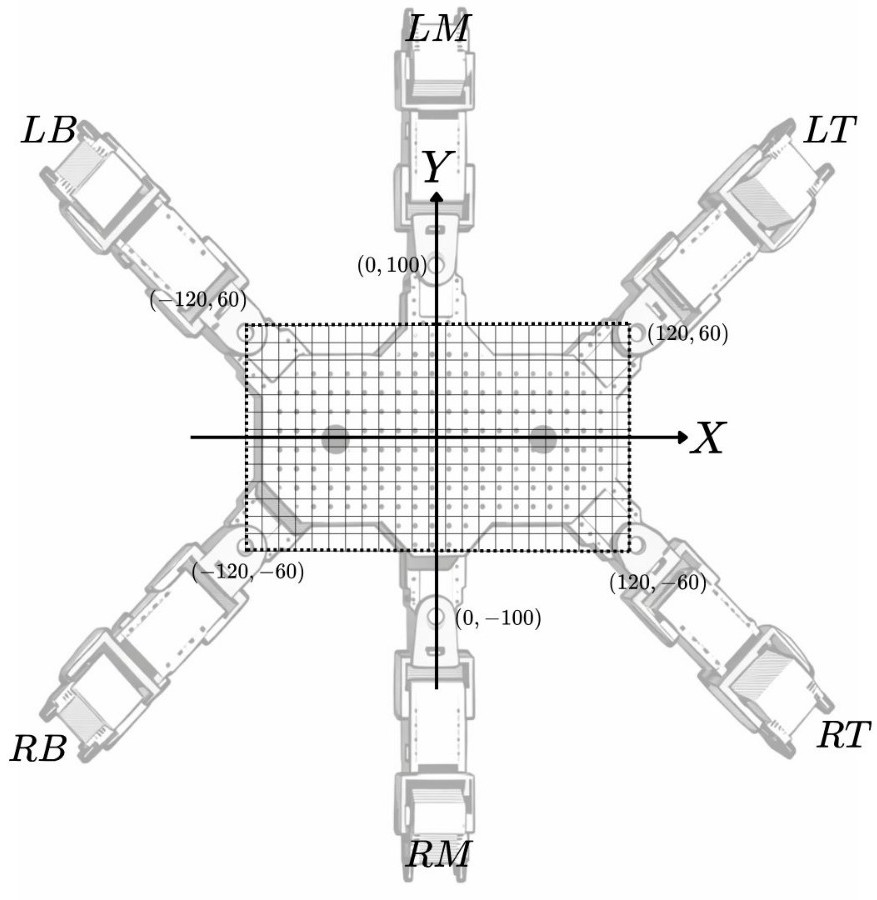
\includegraphics[width=\linewidth]{capitulos/cap2/figuras/coordenadascoxas.jpeg}

        \captionsetup{type=figure}
        \caption[Coordenadas de anclaje de las coxas $(x_i,y_i)$]{Ubicación de los puntos de anclaje de las coxas en el sistema de coordenadas del cuerpo $\{B\}$, expresada mediante las coordenadas planas $(x_i,y_i)$.}
        \label{fig:coordenadascoxas}
        \footnotesize Fuente: Elaboración propia.
    \end{minipage}%
    \hfill%
    \begin{minipage}[t]{0.38\textwidth}
        \vspace{0pt}
        Como ejemplo, si para la pata \textit{Left-Top} (LT) se tiene:
        \begin{equation}
            {}^{B}\bm{p}_{\text{coxa,LT}} =
            \begin{bmatrix}
                120\\ 60\\ 0
            \end{bmatrix}
        \end{equation}

        en el sistema local debe cumplirse ${}^{L_{LT}}\bm{p}_{\text{coxa,LT}}=\bm{0}$. Aplicando la Ec.~\ref{eq:Tlb} a ese punto:
        \begin{equation}
            \bm{0}
            =
            \begin{bmatrix}
                120 + x_j\\
                -60 + y_j\\
                0
            \end{bmatrix}
            \;\Rightarrow\;
            \begin{aligned}
                x_j &= -120,\\
                y_j &= +60.
            \end{aligned}
        \end{equation}

        \vspace{0.5em}

        De forma general, si la posición del eje de la coxa de la pata $i$ en coordenadas del cuerpo es ${}^{B}\bm{p}_{\text{coxa},i}=[x_i\;\;y_i\;\;0]^T$, imponer ${}^{L_i}\bm{p}_{\text{coxa},i}=\bm{0}$ en la Ec.~\ref{eq:Tlb} conduce a:
        \begin{equation}
            \begin{aligned}
                x_j &= -x_i,\\
                y_j &= +y_i.
            \end{aligned}
            \label{eq:xj_yj_general}
        \end{equation}
    \end{minipage}
\end{figure}

\subsection{Matriz de posición del cuerpo y actualización incremental}

La formulación cinemática adoptada en esta subsección sigue el enfoque de control por efectores finales propuesto por Arrigoni et al.~\cite{arrigoni2024control}, expresada aquí con la notación empleada en Craig~\cite{craig2018robotics}. El cuerpo en el espacio global se describe mediante la transformación homogénea ${}^{G}\mathbf{T}_B$, la cual relaciona las coordenadas del sistema del cuerpo $\{B\}$ con el sistema global $\{G\}$. Esta matriz se actualiza recursivamente en cada iteración $i$, integrando dos componentes: (i) el movimiento acumulado por el generador de marcha (Secciones~\ref{subsec:gaits} y~\ref{subsec:trajectory_planning}), y (ii) las consignas de posición (traslación y rotación) definidas por el usuario.

En el instante inicial ($i=0$), la transformación global-cuerpo se define como una traslación pura en el eje $Z$, situando al robot a su altura inicial $SP_z$:

\vspace{-0.5\baselineskip}
\begin{equation}
    {}^{G}\mathbf{T}_{B,0} =
    \begin{bmatrix}
        \mathbf{I}_{3\times 3} & {}^{G}\bm{p}_{B,0}\\
        \bm{0}_{1\times 3} & 1
    \end{bmatrix},
    \quad \text{con} \quad
    {}^{G}\bm{p}_{B,0} =
    \begin{bmatrix}
        0 \\ 0 \\ SP_z
    \end{bmatrix}.
    \label{eq:Tgb0}
\end{equation}
\vspace{-0.8\baselineskip}

En cada iteración $i$, la matriz de estado ${}^{G}\mathbf{T}_{B,i}$ se construye mediante la composición de transformaciones:

\vspace{-1\baselineskip}
\begin{equation}
    {}^{G}\mathbf{T}_{B,i}
    =
    \mathbf{T}_{tr,i} \cdot \mathbf{M}_{ov,i} \cdot \left( \mathbf{R}_{z,i}\,\mathbf{R}_{y,i}\,\mathbf{R}_{x,i} \right).
    \label{eq:Tgb_decomp_full}
\end{equation}

Aquí, $\mathbf{T}_{tr,i}$ representa la localización odométrica del robot en la iteración $i$: la posición en el plano, la orientación en \textit{yaw} y la altura base que resultan de acumular, desde el instante inicial, los desplazamientos producidos por la marcha. Se calcula recursivamente aplicando el incremento de movimiento $\mathbf{Q}_{tr,i}$ calculado por el generador de marcha:

\vspace{-1\baselineskip}
\begin{equation}
    \mathbf{T}_{tr,i} = \mathbf{T}_{tr,i-1} \; \mathbf{Q}_{tr,i},
    \label{eq:Ttr_rec}
\end{equation}
\vspace{-1.0\baselineskip}

donde el incremento $\mathbf{Q}_{tr,i}$ se descompone en una traslación y una rotación diferencial en el eje vertical. Por tanto, $\mathbf{Q}_{tr,i}$ no representa la posición completa del cuerpo, sino únicamente la aportación incremental de la marcha a la trayectoria acumulada:

\vspace{-0.5\baselineskip}
\begin{equation}
    \mathbf{Q}_{tr,i} = 
    \underbrace{
    \begin{bmatrix}
        1 & 0 & 0 & \delta x_{gait,i} \\
        0 & 1 & 0 & \delta y_{gait,i} \\
        0 & 0 & 1 & 0 \\
        0 & 0 & 0 & 1
    \end{bmatrix}
    }_{\delta\mathbf{T}_{mov,i}}
    \cdot
    \underbrace{
    \begin{bmatrix}
        \cos(\delta rot_{z_{i}}) & -\sin(\delta rot_{z_{i}}) & 0 & 0 \\
        \sin(\delta rot_{z_{i}}) & \cos(\delta rot_{z_{i}})  & 0 & 0 \\
        0 & 0 & 1 & 0 \\
        0 & 0 & 0 & 1
    \end{bmatrix}
    }_{\delta\mathbf{R}_{z,i}}
    \label{eq:Qtr}
\end{equation}
\vspace{-0.5\baselineskip}

Por otra parte, la posición del cuerpo se gestiona componiendo la traslación relativa $\mathbf{M}_{ov,i}$ y la secuencia de rotaciones Euler $ZYX$: 

\begin{equation}
    \renewcommand{\arraystretch}{1.3} % Ajusta el espacio vertical para que no se vea apretado
    \mathbf{M}_{ov,i} \cdot \left( \mathbf{R}_{z,i}\,\mathbf{R}_{y,i}\,\mathbf{R}_{x,i} \right)
    =
    \left[
    \begin{array}{c|c}
      \mathbf{R}_{z}(\alpha_i)\,\mathbf{R}_{y}(\beta_i)\,\mathbf{R}_{x}(\gamma_i) & 
      \begin{matrix}
         \mathrm{bodyPos}_{x,i} \\ 
         \mathrm{bodyPos}_{y,i} \\ 
         \mathrm{bodyPos}_{z,i}
      \end{matrix} \\
      \hline
      \mathbf{0}_{1\times 3} & 1
    \end{array}
    \right]
    \label{eq:T_user_compact}
\end{equation}

Sobre esta composición podría añadirse, además, una transformación de estabilización actualizada mediante retroalimentación sensorial.

\subsubsection{Incremento de movimiento del cuerpo: $\mathbf{Q}_{body,i}$}

Para actualizar la posición del efector final durante la fase de apoyo, no basta con conocer la posición absoluta del chasis; también es necesario cuantificar cómo cambia entre dos instantes de control consecutivos, $i-1$ y $i$. Siguiendo esta formulación, se define la transformación diferencial $\mathbf{Q}_{body,i}$, que expresa el sistema actual $\{B_i\}$ respecto al sistema anterior $\{B_{i-1}\}$~\cite{arrigoni2024control}:

\vspace{-1\baselineskip}
\begin{equation}
    \mathbf{Q}_{body,i} = \left({}^{G}\mathbf{T}_{B,i-1}\right)^{-1} \cdot {}^{G}\mathbf{T}_{B,i}
    \label{eq:Qbody_def_full}
\end{equation}

En otras palabras, $\mathbf{Q}_{body,i}$ representa el movimiento relativo completo del cuerpo entre dos iteraciones consecutivas. Esta magnitud es la que permite actualizar las posiciones de apoyo de forma recursiva e imponer la condición de no deslizamiento. Conviene distinguirla de $\mathbf{Q}_{tr,i}$: mientras esta última modela solamente el incremento odométrico de la marcha, $\mathbf{Q}_{body,i}$ recoge el cambio efectivo de la posición completa del chasis entre $i-1$ e $i$.

\subsection{Actualización de los efectores finales}

\subsubsection{Fase de apoyo (\textit{stance})}

Durante la fase de apoyo (\textit{stance}), la hipótesis fundamental es que el pie no desliza sobre el terreno. Esto implica que la posición del efector final de la pata es constante en el sistema global $\{G\}$:

\vspace{-0.5\baselineskip}
\begin{equation}
    {}^{G}\bm{p}_{foot, i} = {}^{G}\bm{p}_{foot, i-1} = \text{cte}
\end{equation}

Sin embargo, el chasis sí se desplaza y rota entre iteraciones. Por tanto, aun cuando el efector final de la pata permanezca inmóvil en el sistema global $\{G\}$, sus coordenadas expresadas en el sistema del cuerpo $\{B\}$ cambian, porque el propio sistema $\{B\}$ se ha movido. Bajo esta hipótesis, la actualización recursiva de los efectores finales en apoyo se expresa como~\cite{arrigoni2024control}:

\vspace{-0.5\baselineskip}
\begin{equation}
    {}^{B}{\bm{p}}_{foot,i}
    =
    \left( \mathbf{Q}_{body,i} \right)^{-1} \cdot {}^{B}{\bm{p}}_{foot,i-1}
    \label{eq:stance_update}
\end{equation}

Al tratarse de una relación recursiva, es necesario definir la condición inicial ${}^{B}{\bm{p}}_{foot,0}$ para iniciar el proceso iterativo. La condición inicial del movimiento se toma en la \textbf{postura neutral}, definida en la Tabla~\ref{tab:neutral_positions}; no debe confundirse con el inicio de cada fase de apoyo, cuya posición viene dada por el final del vuelo anterior.

\vspace{-0.5\baselineskip}
\begin{table}[H]
    \centering
    \captionsetup{justification=centering}
    \caption{Coordenadas de la postura neutral (${}^{B}\bm{p}_{neu}$) configuradas para cada extremidad en el sistema de referencia del cuerpo.}
    \label{tab:neutral_positions}
    \begin{tabular}{lrrr}
        \toprule
        \textbf{Pata} & \textbf{X [mm]} & \textbf{Y [mm]} & \textbf{Z [mm]} \\
        \midrule
        Izquierda Delantera (LT) & $+180$ & $+170$ & $-100$ \\
        Izquierda Media (LM)     & $0$    & $+240$ & $-100$ \\
        Izquierda Trasera (LB)   & $-180$ & $+170$ & $-100$ \\
        Derecha Trasera (RB)     & $-180$ & $-170$ & $-100$ \\
        Derecha Media (RM)       & $0$    & $-240$ & $-100$ \\
        Derecha Delantera (RT)   & $+180$ & $-170$ & $-100$ \\
        \bottomrule
    \end{tabular}
\end{table}

\subsubsection{Fase de transferencia (\textit{swing}) y continuidad del ciclo}

Durante la fase de transferencia (\textit{swing}), el pie se eleva y se desplaza hasta el siguiente punto de apoyo. Este movimiento se describe en el sistema de trayectoria $\{tr\}$, cuya posición y orientación respecto a $\{G\}$ vienen dadas por $\mathbf{T}_{tr,i}$. El punto de despegue ${}^{tr}\bm{p}^{-}$ se obtiene expresando en este sistema la posición calculada del pie al finalizar el apoyo.

\begin{wrapfigure}[15]{r}{0.6\textwidth}
    \vspace{-0.5\baselineskip}
    \centering
    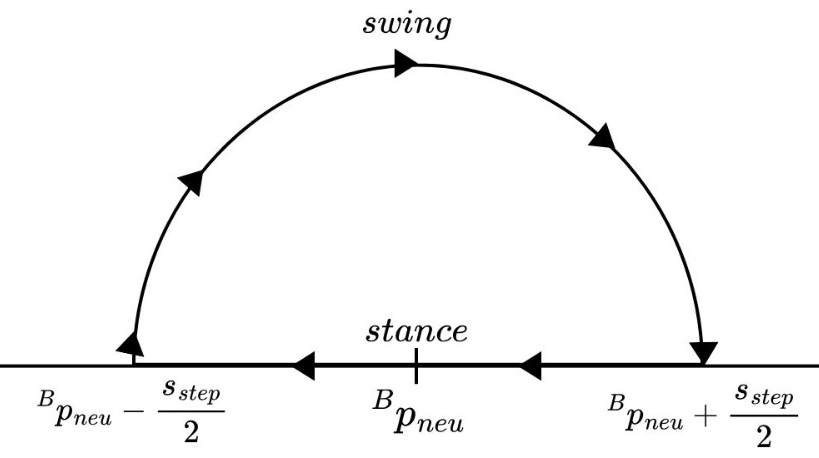
\includegraphics[width=\linewidth]{capitulos/cap2/figuras/continuidad.jpeg}
    \captionsetup{justification=centering}
    \caption[Esquema de continuidad del ciclo de paso]{Ciclo del pie respecto al cuerpo con traslación constante.}
    \label{fig:diagrama_continuidad_ciclo}
    {\footnotesize Fuente: Elaboración propia.}
    \vspace{-0.5\baselineskip}
\end{wrapfigure}

El paso $\bm{s}_{step}$ es el desplazamiento horizontal del cuerpo durante una fase de apoyo (Subsección~\ref{subsec:gait_parameters}). Si el pie aterriza medio paso por delante de la postura neutral, el avance del cuerpo durante el apoyo lo sitúa, respecto al chasis, medio paso por detrás de ella. Así, el recorrido queda centrado en la postura neutral, como muestra la Figura~\ref{fig:diagrama_continuidad_ciclo}.

Cuando la marcha combina traslación y giro, el destino se calcula como ${}^{tr}\bm{p}^{+}=\mathbf{R}_{gait}\mathbf{T}_{step}\,{}^{B}\bm{p}_{neu}$. La transformación $\mathbf{T}_{step}$ desplaza la posición neutral $\bm{s}_{step}/2$, y $\mathbf{R}_{gait}$ aplica a continuación una rotación alrededor del eje vertical igual a la mitad del giro previsto durante el apoyo. Las coordenadas de despegue y aterrizaje se almacenan en ese instante y se mantienen constantes durante el vuelo. Entre ellas se define la trayectoria:

\vspace{-0.5\baselineskip}
\begin{equation}
    {}^{tr}\bm{p}_{traj}(u)
    = {}^{tr}\bm{p}^{-}
    + f_{xy}(u)\left({}^{tr}\bm{p}^{+}-{}^{tr}\bm{p}^{-}\right),
    \qquad u\in[0,1].
    \label{eq:swing_latched_interp}
\end{equation}
\vspace{-1\baselineskip}

La variable $u$ representa el progreso del vuelo, desde el despegue ($u=0$)
hasta el aterrizaje ($u=1$), y $f_{xy}(u)$ es la función de interpolación descrita en la Subsección~\ref{subsec:theory_swing}. En cada iteración $i$, esta trayectoria se transforma al sistema global y se le añade la elevación vertical $\Delta z_{step}(u)$:

\vspace{-0.5\baselineskip}
\begin{equation}
    {}^{G}\bm{p}_{swing,i}
    = \mathbf{T}_{tr,i}\,{}^{tr}\bm{p}_{traj}(u_i)
    + \Delta z_{step}(u_i)\,\hat{Z}_G.
    \label{eq:swing_global_calc}
\end{equation}
\vspace{-1\baselineskip}

El término $\Delta z_{step}(u)$, definido en la Subsección~\ref{subsec:theory_swing}, proporciona la elevación del pie en la dirección vertical global $\hat{Z}_G$, anulándose al despegar y al aterrizar. Un futuro mapa de elevación $h({}^{G}p_x,{}^{G}p_y)$ permitiría ajustar la cota de aterrizaje y el perfil vertical de vuelo a la geometría del terreno.

Finalmente, la referencia se expresa en el sistema del cuerpo $\{B\}$:

\vspace{-0.5\baselineskip}
\begin{equation}
    {}^{B}\bm{p}_{swing,i}
    = \left({}^{G}\mathbf{T}_{B,i}\right)^{-1}\,{}^{G}\bm{p}_{swing,i}.
    \label{eq:swing_body_transform}
\end{equation}
\vspace{-1\baselineskip}

La continuidad de posición entre fases se establece tomando como despegue el final del apoyo anterior y como inicio del siguiente apoyo el final del vuelo. Si la consigna de desplazamiento cambia durante la transferencia, los extremos almacenados en $\{tr\}$ no se recalculan, ya que el nuevo valor se incorpora al planificar el destino del siguiente vuelo. 



\section{Modelado cinemático inverso}

\subsection{Concepto de cinemática inversa}

La cinemática inversa (IK, por sus siglas en inglés, \textit{Inverse Kinematics}) aborda el problema de determinar la configuración articular $\bm{q}$ necesaria para alcanzar un objetivo cartesiano. En este TFG, el efector final se especifica únicamente por su posición $\bm{P}$ en el espacio. El proceso se denota como $\bm{q} = f^{-1}(\bm{P})$. A diferencia de la cinemática directa, este cálculo es no lineal, pudiendo presentar múltiples soluciones para un mismo punto objetivo \cite{craig2018robotics,siciliano2016springer}.

Si bien en manipuladores complejos es frecuente recurrir a métodos numéricos iterativos, estos resultan inadecuados para sistemas embebidos de tiempo real debido a su alto coste computacional y problemas de convergencia. Sin embargo, para cadenas cinemáticas de pocos grados de libertad, como la extremidad de este hexápodo (3-DOF), es posible obtener soluciones analíticas exactas mediante dos enfoques:

\begin{enumerate}
    \item \textbf{Solución Algebraica:} Se basa en seguir la convención Denavit-Hartenberg, para despejar las variables articulares. Aunque riguroso, suele generar expresiones complejas y operaciones matriciales costosas.
    
    \item \textbf{Solución Geométrica:} Aprovecha la implementación física del mecanismo para descomponer el problema espacial 3D en problemas planos 2D más sencillos, resolviéndolos mediante trigonometría. En este TFG se ha optado por este enfoque.
\end{enumerate}


\vspace{-1\baselineskip}
\subsection{Parámetros geométricos}

La pata se modela como una cadena cinemática abierta de tres eslabones rígidos (coxa, fémur y tibia), de longitudes constantes $L_c$, $L_f$ y $L_t$. Para formular la cinemática inversa se define un sistema de referencia local de pata $\{L\}$ en la articulación de la coxa. La convención adoptada mantiene $X_L$ alineado con $X_B$, sitúa $Y_L$ perpendicular a $X_L$ en el plano horizontal y con sentido opuesto a $Y_B$, y define $Z_L$ positivo hacia abajo, en sentido opuesto a $Z_B$. Por tanto, $Y_L$ no coincide necesariamente con la dirección radial de cada pata; su orientación particular respecto al chasis se incorpora mediante el ángulo fijo de montaje $\varepsilon_i$ en el cálculo de la coxa. Esta configuración de 3 Grados de Libertad permite posicionar el efector final dentro del espacio de trabajo de la extremidad. La Figura~\ref{fig:frame_pata_tikz} resume esta definición junto con las dimensiones nominales de los eslabones.

\begin{figure}[!ht]
    \centering
    \begin{minipage}[c]{0.64\textwidth}
        \centering
        \resizebox{\linewidth}{!}{%
        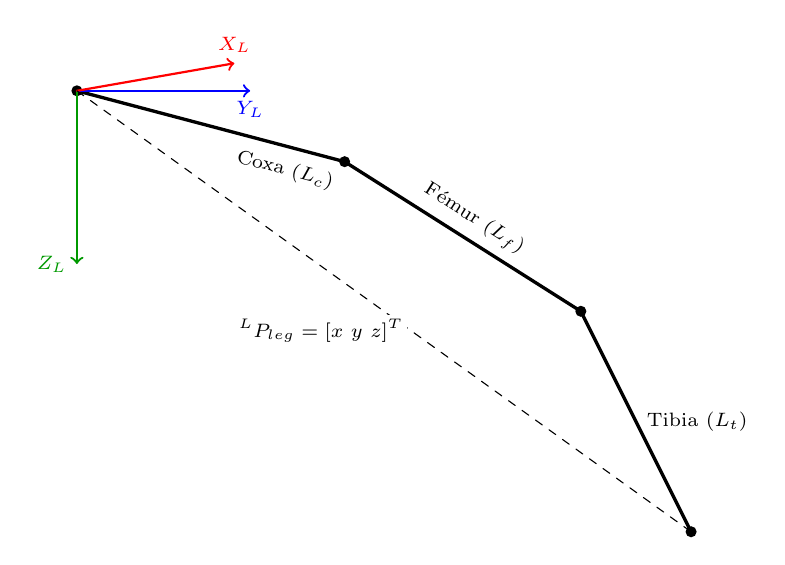
\begin{tikzpicture}[
            x=1cm,
            y=-1cm,
            line cap=round,
            line join=round,
            every node/.style={font=\scriptsize}
        ]
            % --- Puntos (esquema 2D: plano Y-Z; Z positivo hacia abajo) ---
            \coordinate (O) at (0,0);
            \coordinate (K) at (3.4,0.9);
            \coordinate (A) at (6.4,2.8);
            \coordinate (F) at (7.8,5.6);

            % --- Eslabones ---
            \draw[very thick] (O) -- (K) node[pos=0.80, below, sloped, yshift=-1pt] {Coxa ($L_c$)};
            \draw[very thick] (K) -- (A) node[midway, above, sloped] {Fémur ($L_f$)};
            \draw[very thick] (A) -- (F) node[midway, right] {Tibia ($L_t$)};

            % --- Articulaciones (sin etiquetas) ---
            \fill (O) circle (2.0pt);
            \fill (K) circle (2.0pt);
            \fill (A) circle (2.0pt);
            \fill (F) circle (2.0pt);

            % --- Ejes del frame {L} ---
            \draw[->, thick, blue] (O) -- ++(2.2,0) node[below] {$Y_L$};
            \draw[->, thick, green!60!black] (O) -- ++(0,2.2) node[left] {$Z_L$};
            \draw[->, thick, red] (O) -- ++(2.0,-0.35) node[above] {$X_L$};

            % --- Vector objetivo ---
            \draw[dashed] (O) -- (F);
            \node[fill=white, inner sep=1.5pt] at (3.1,3.05) {${}^{L}\bm{P}_{leg}=[x\ y\ z]^T$};
        \end{tikzpicture}%
        }
    \end{minipage}
    \hfill
    \begin{minipage}[c]{0.33\textwidth}
        \captionsetup{type=figure}
        \caption[Sistema local y estructura de la pata]{Sistema local de pata $\{L\}$ y longitudes $L_c$, $L_f$ y $L_t$.}
        \label{fig:frame_pata_tikz}
        \footnotesize Fuente: Elaboración propia.

        \vspace{0.75em}
        \centering
        \small
        \textbf{Longitudes nominales}\\[0.35em]
        \begin{tabular}{@{}lr@{}}
            \toprule
            \textbf{Eslabón} & \textbf{$L$ (mm)} \\
            \midrule
            Coxa  & 52  \\
            Fémur & 66  \\
            Tibia & 135 \\
            \bottomrule
        \end{tabular}
    \end{minipage}

\end{figure}


\subsection{Resolución de la cinemática inversa (IK)}
\label{subsec:theory_ik}

El objetivo de la Cinemática Inversa consiste en determinar el vector de variables articulares:
\begin{equation}
    \bm{q} =
    \begin{bmatrix}
        \theta_{\text{coxa}} \\ \theta_{\text{femur}} \\ \theta_{\text{tibia}}
    \end{bmatrix}
\end{equation}

de manera que la punta de la pata alcance la coordenada objetivo ${}^{L}\bm{P}_{leg}$. Dado que los ejes de rotación del fémur y la tibia son paralelos entre sí, y ortogonales al eje de la coxa, el problema espacial 3D puede desacoplarse en: (i) un problema plano en el plano horizontal para la coxa, y (ii) un problema plano de dos eslabones en el plano vertical.


A continuación se presentan (y se deducen) las ecuaciones para la pata \textit{Left-Top}. El resto de patas se obtienen aplicando la misma formulación y ajustando los offsets de montaje (traslaciones y el offset angular $\varepsilon_i$) propios de cada anclaje.

\textbf{1) Cálculo del ángulo de Coxa ($\theta_{\text{coxa}}$):}

Sea el objetivo cartesiano expresado en el sistema local de pata $\{L\}$ como ${}^{L}\bm{P}_{leg}=[x\ y\ z]^T$. La orientación de la coxa viene determinada por la proyección de dicho objetivo sobre el plano horizontal $X_LY_L$. Adoptando la convención de signos de la Figura~\ref{fig:ik_coxa}, el ángulo se obtiene como:

\vspace{-1\baselineskip}
\begin{equation}
    \theta_{\text{coxa}} = -\operatorname{atan2}(y, x) - \varepsilon_i
    \label{eq:ik_theta}
\end{equation}
\vspace{-1\baselineskip}

\begin{figure}[H]
    \centering
    \begin{minipage}[c]{0.72\textwidth}
        \centering
        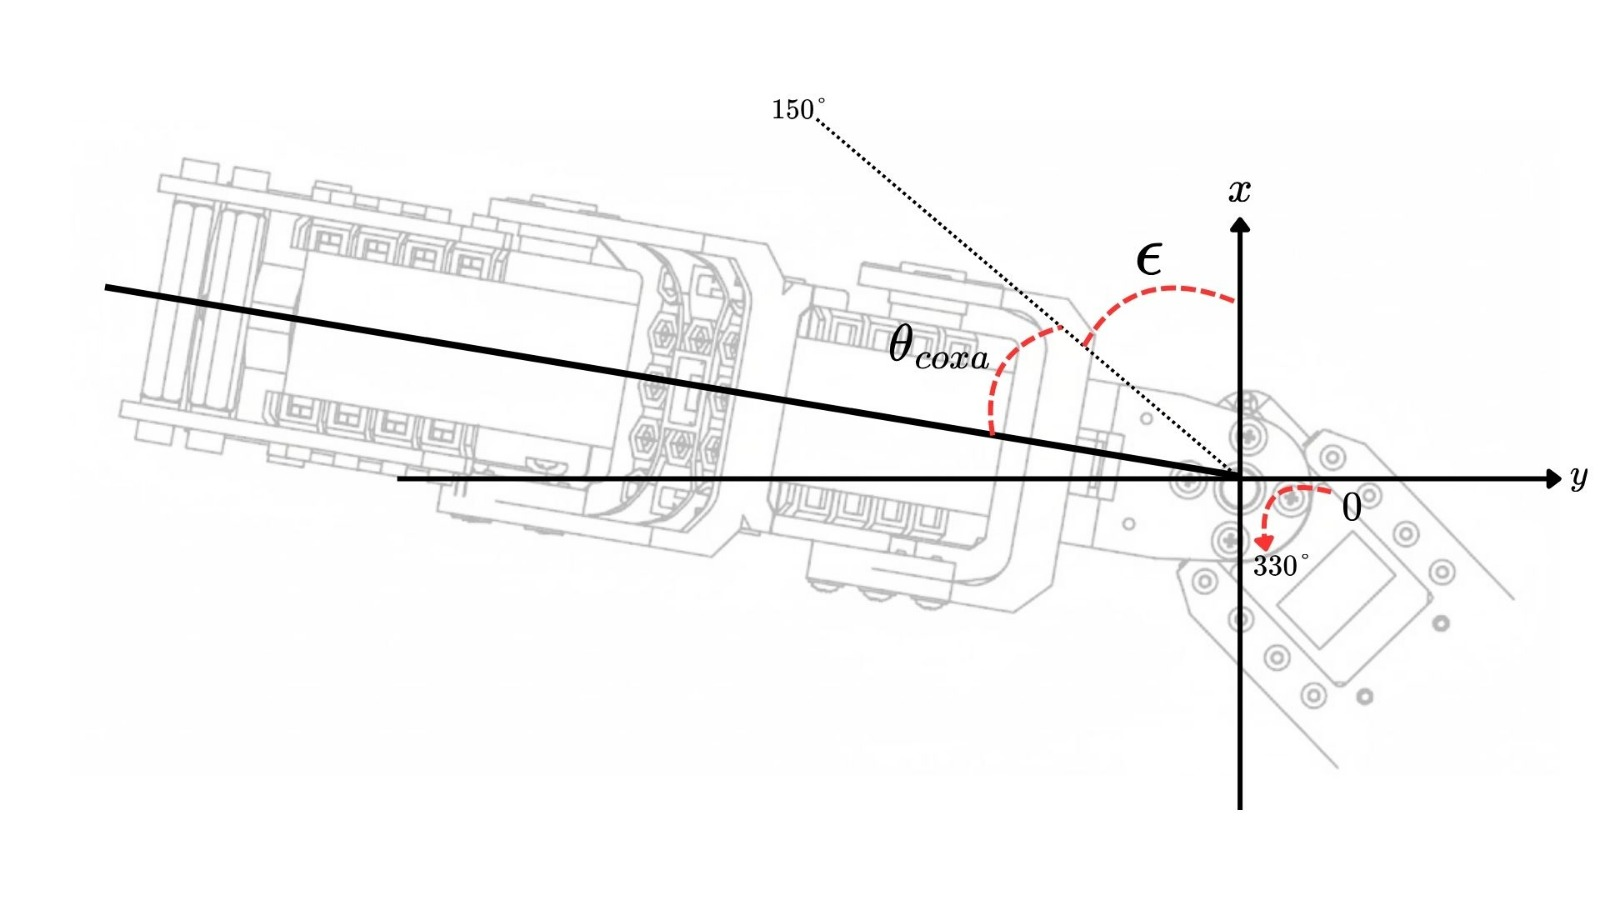
\includegraphics[width=\linewidth]{capitulos/cap2/figuras/coxa.jpeg}
    \end{minipage}
    \hfill
    \begin{minipage}[c]{0.20\textwidth}
        \centering
        \scriptsize
        \setlength{\tabcolsep}{5pt}
        \renewcommand{\arraystretch}{1.0}
        \textbf{Valores de $\varepsilon_i$}\\[0.25em]
        \begin{tabular}{@{}lc@{}}
            \toprule
            \textbf{Pata} & \textbf{$\varepsilon_i$} \\
            \midrule
            LT & $+45^\circ$  \\
            LM & $+90^\circ$  \\
            LB & $+135^\circ$ \\
            RT & $-45^\circ$  \\
            RM & $-90^\circ$  \\
            RB & $-135^\circ$ \\
            \bottomrule
        \end{tabular}
    \end{minipage}
    \caption[Cálculo del ángulo de coxa]{Geometría usada para el cálculo del ángulo de coxa en el plano $X_LY_L$}
    \label{fig:ik_coxa}
    {\footnotesize Fuente: Elaboración propia.}
\end{figure}

donde $\varepsilon_i$ representa el \textbf{offset angular de montaje} de la pata, medido desde el eje longitudinal $X_B$ del chasis y positivo en sentido antihorario visto desde arriba, es decir, hacia $+Y_B$. Se trata de un ángulo constante en cada pata; sus valores se recogen de forma resumida junto a la figura y, junto con los signos de giro y ajustes de montaje, en la Tabla~\ref{tab:parametros_pata}. A diferencia de $\arctan\left(\tfrac{y}{x}\right)$, la función $\operatorname{atan2}(y,x)$ resuelve correctamente la ambigüedad de cuadrantes y cubre el rango completo $(-\pi,\pi]$, por lo que es la forma recomendada en la implementación.

Después de aplicar el offset $\varepsilon_i$, el resultado se normaliza de
nuevo al intervalo $[-\pi,\pi]$ mediante
$\operatorname{atan2}(\sin\theta_{\text{coxa}},
\cos\theta_{\text{coxa}})$. Esta operación no modifica la orientación de la
articulación, pero evita representaciones equivalentes con vueltas completas,
como $310^\circ$ en lugar de $-50^\circ$, que producirían una consigna
incorrecta al añadir el offset del servomotor.


\textbf{2) Cálculo de los ángulos de fémur y tibia (mecanismo plano fémur--tibia):}\par\medskip

Una vez determinada la orientación de la coxa ($\theta_{coxa}$), dado que los ejes de rotación del fémur y la tibia son paralelos entre sí y perpendiculares al plano de movimiento definido por la coxa, el sistema puede reducirse a un \textbf{mecanismo plano de dos eslabones}, como se muestra en la Figura~\ref{fig:ik_femur_tibia}:

\vspace{-1\baselineskip}
\begin{figure}[H]
    \centering

    \begin{minipage}[c]{0.72\textwidth}
        \centering
        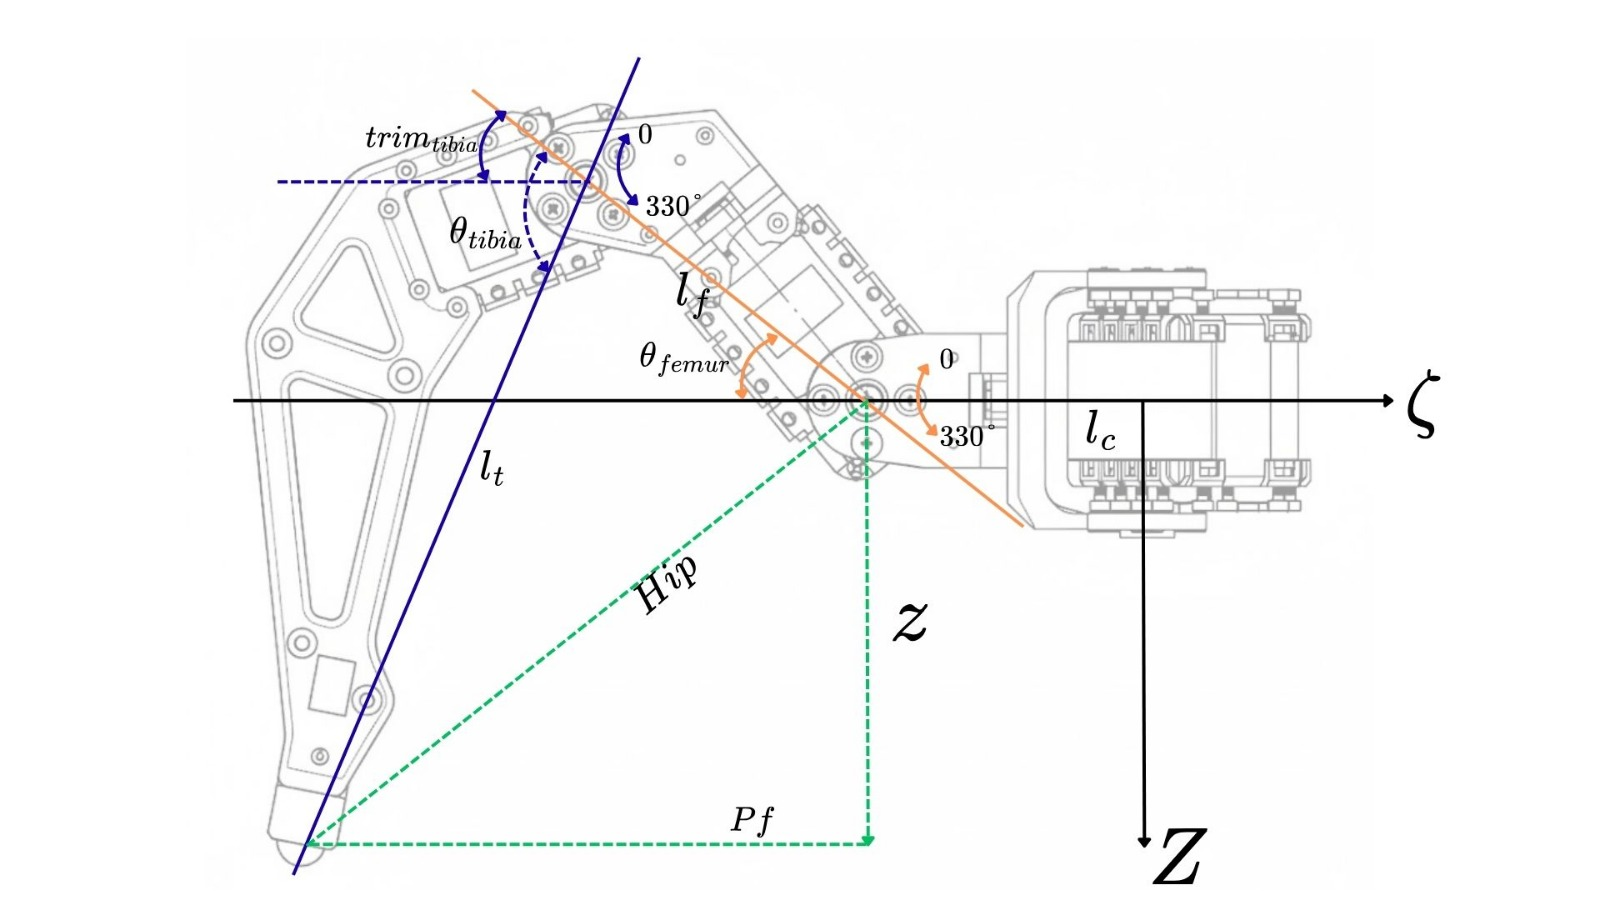
\includegraphics[width=\linewidth]{capitulos/cap2/figuras/femur_tibia.jpeg}
    \end{minipage}
    \hfill
    \begin{minipage}[c]{0.24\textwidth}
        \captionsetup{type=figure,justification=raggedright,singlelinecheck=false}
        \caption[Reducción al mecanismo plano fémur--tibia]{Geometría del mecanismo plano fémur--tibia.}
        \label{fig:ik_femur_tibia}
        \footnotesize Fuente: Elaboración propia.
    \end{minipage}
\end{figure}
\vspace{-1\baselineskip}

La distancia horizontal desde la articulación del fémur hasta la proyección del efector final, denominada $P_f$, se obtiene restando la longitud de la coxa ($L_c$) a la magnitud radial total en el plano $XY$. Asimismo, se define la distancia directa (hipotenusa virtual) que conecta la articulación del hombro (fémur) con la punta de la pata, denotada como $Hip$:

\noindent
\begin{minipage}[t]{0.47\textwidth}
\begin{equation}
    P_f = \sqrt{x^2 + y^2} - L_c
    \label{eq:trueX}
\end{equation}
\end{minipage}
\hfill
\begin{minipage}[t]{0.48\textwidth}
\begin{equation}
    Hip = \sqrt{P_f^2 + z^2}
    \label{eq:im_dist}
\end{equation}
\end{minipage}


Conocidas las tres longitudes del triángulo ($L_f$ del fémur, $L_t$ de la tibia y la distancia virtual $Hip$), es posible obtener los ángulos articulares por el teorema del coseno.

\paragraph{Ángulo del fémur ($\theta_{\text{femur}}$)}:
El ángulo objetivo del fémur se compone de dos partes: la elevación del vector $Hip$ respecto a la horizontal y el ángulo interno del triángulo ($\alpha_1$) adyacente a la articulación.

\vspace{-1\baselineskip}
\begin{equation}
    \theta_{\text{femur}} = \frac{\pi}{2} - \operatorname{atan2}(P_f,\, z) - \arccos\!\left(\frac{L_f^2 + Hip^2 - L_t^2}{2 \cdot L_f \cdot Hip}\right)
    \label{eq:theta_femur}
\end{equation}
\vspace{-1\baselineskip}

\paragraph{Ángulo de la tibia ($\theta_{\text{tibia}}$)}:
El ángulo de la tibia determina la flexión de la rodilla y se deriva del ángulo interno ($\beta$) opuesto al lado $Hip$.

\vspace{-1\baselineskip}
\begin{equation}
    \theta_{\text{tibia}} = \pi - \arccos\left(\frac{L_f^2 + L_t^2 - Hip^2}{2 \cdot L_f \cdot L_t}\right)
    \label{eq:theta_tibia}
\end{equation}
\vspace{-1\baselineskip}

La tibia requiere además un ajuste propio: a diferencia de un modelo ideal, donde el ángulo cero corresponde a una extensión perfecta, el servo se monta de forma no colineal con el eje del eslabón, por lo que se introduce un offset angular de montaje que se incorpora en la Ec.~\ref{eq:calibracion_theta_servo}.

\subsubsection{Ajuste y transformación a grados}
\label{subsec:ajuste_transformacion_grados}

La IK geométrica proporciona ángulos articulares en radianes, referenciados al cero geométrico de cada articulación. Sin embargo, estos valores no pueden enviarse directamente a los servomotores: deben transformarse al sistema angular del actuador incorporando el sentido efectivo de giro y los ajustes de montaje. De forma esquemática, el proceso que conduce desde la posición objetivo del pie hasta la consigna articular final puede resumirse como:

\vspace{-1.5\baselineskip}
\begin{equation}
    {}^{B}\bm{p}_{foot,i}
    \;\xrightarrow{\text{BODY}\rightarrow\text{LEG}}\;
    {}^{L_i}\bm{p}_{foot,i}
    \;\xrightarrow{\text{IK}}\;
    \begin{bmatrix}\theta_{\text{coxa}} \\ \theta_{\text{femur}} \\ \theta_{\text{tibia}}\end{bmatrix}_i
    \;\xrightarrow{\text{Ec.}\,\ref{eq:calibracion_theta_servo}}\;
    \begin{bmatrix}\theta_{cmd,c} \\ \theta_{cmd,f} \\ \theta_{cmd,t}\end{bmatrix}_i
    \label{eq:pipeline_completo}
\end{equation}
\vspace{-0.5\baselineskip}

De manera general, la transformación final puede escribirse como:

\vspace{-1\baselineskip}
\begin{equation}
    \theta_{cmd}
    =
    \theta_0 + \text{trim} + s\,\theta_{IK}
    \label{eq:calibracion_theta_servo}
\end{equation}
\vspace{-1.0\baselineskip}

donde $\theta_0$ representa la referencia angular del actuador, $s\in\{+1,-1\}$ introduce el sentido efectivo de giro y $\text{trim}$ compensa los desajustes derivados del montaje. En la configuración adoptada, coxa y fémur no requieren corrección adicional, mientras que la tibia incorpora un ajuste fijo de $\pm 45^\circ$ asociado a su geometría de anclaje. No se establecen límites mecánicos particulares por articulación, ya que estos deben obtenerse experimentalmente para el montaje construido. La Figura~\ref{fig:cuerpo_ajuste_grados} muestra el hexápodo completo con los sistemas de coordenadas definidos en todas las patas, y los valores concretos empleados en cada una se resumen en la Tabla~\ref{tab:parametros_pata}.

\vspace{-1.0\baselineskip}
\begin{center}
    \begin{minipage}[t]{1\textwidth}
        \centering
        \captionsetup{type=figure,justification=centering,singlelinecheck=false,skip=3pt}
        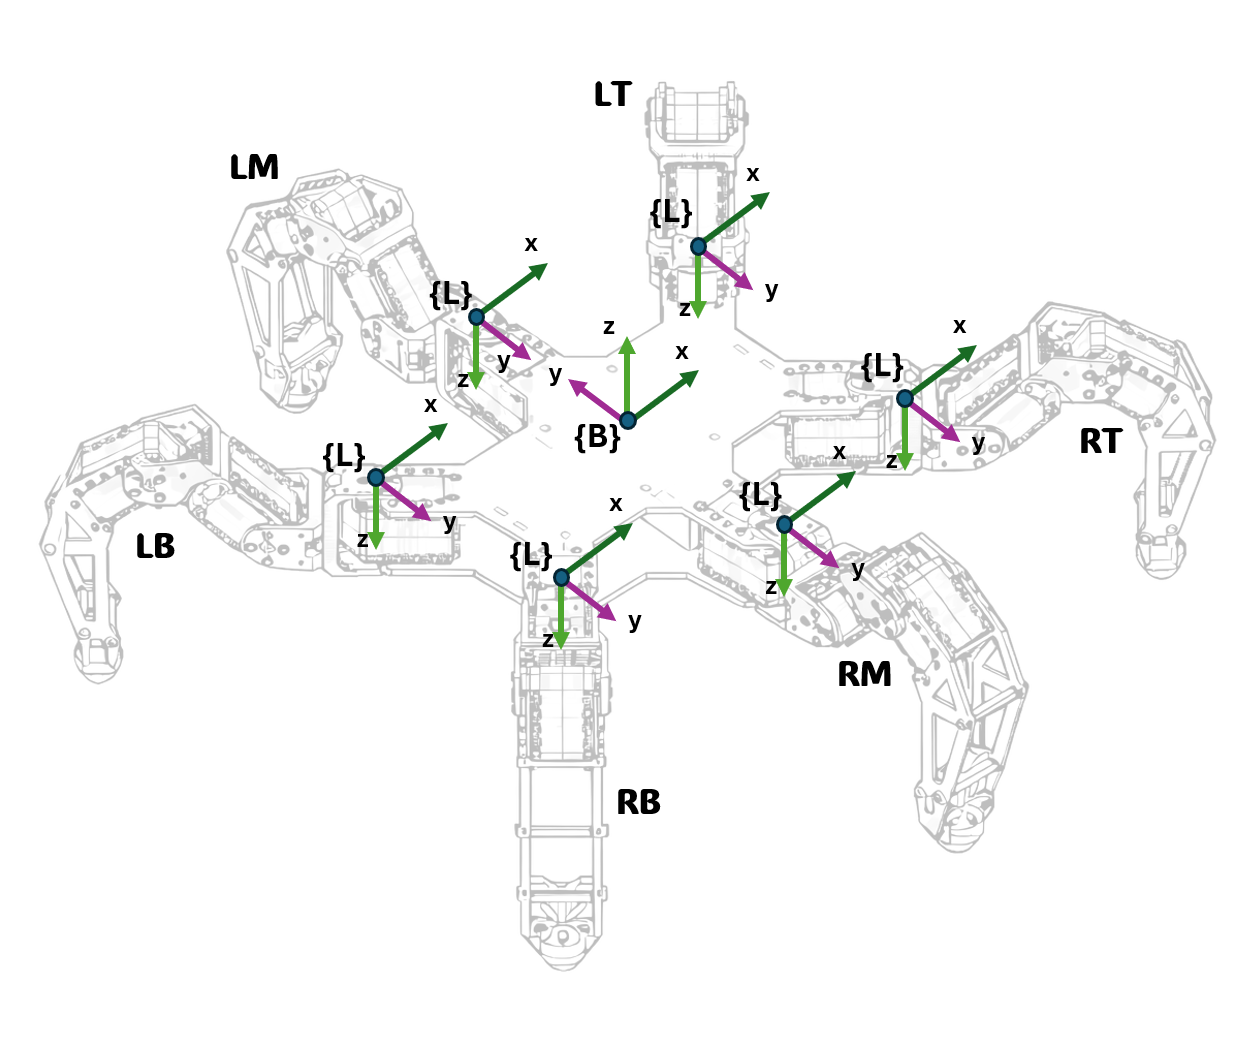
\includegraphics[width=\linewidth,height=0.305\textheight,keepaspectratio]{capitulos/cap2/figuras/CUERPO FRAMES.png}
        \captionof{figure}[Esquema de ajuste y conversión a grados]{Esquema del hexápodo con los sistemas de coordenadas definidos en todas las patas.}
        \label{fig:cuerpo_ajuste_grados}
        \par{\footnotesize Fuente: Elaboración propia.}
    \end{minipage}
\end{center}


\begin{center}
    \setlength{\tabcolsep}{5pt}
    \renewcommand{\arraystretch}{1.05}
    \begin{minipage}[t]{0.88\textwidth}
        \centering
        \small
        \captionsetup{type=table, justification=centering, skip=3pt}
        \begin{minipage}[t]{0.45\textwidth}
            \centering
            \scriptsize\textbf{Patas izquierdas}\\[0.35em]
            \begin{tabular}{@{}lccc@{}}
                \toprule
                \textbf{Pata} & \textbf{$\varepsilon_i$} & \textbf{signos} & \textbf{$\text{trim}_{t}$} \\
                \midrule
                LT & $+45^\circ$  & $(+1,+1,+1)$ & $-45^\circ$ \\
                LM & $+90^\circ$  & $(+1,+1,+1)$ & $-45^\circ$ \\
                LB & $+135^\circ$ & $(+1,+1,+1)$ & $-45^\circ$ \\
                \bottomrule
            \end{tabular}
        \end{minipage}
        \hfill
        \begin{minipage}[t]{0.45\textwidth}
            \centering
            \scriptsize\textbf{Patas derechas}\\[0.35em]
            \begin{tabular}{@{}lccc@{}}
                \toprule
                \textbf{Pata} & \textbf{$\varepsilon_i$} & \textbf{signos} & \textbf{$\text{trim}_{t}$} \\
                \midrule
                RT & $-45^\circ$  & $(+1,-1,-1)$ & $+45^\circ$ \\
                RM & $-90^\circ$  & $(+1,-1,-1)$ & $+45^\circ$ \\
                RB & $-135^\circ$ & $(+1,-1,-1)$ & $+45^\circ$ \\
                \bottomrule
            \end{tabular}
        \end{minipage}

        \vspace{0.4em}
        \captionof{table}[Parámetros geométricos y de montaje]{Parámetros geométricos y de montaje.}
        \label{tab:parametros_pata}
    \end{minipage}
\end{center}

\section{Algoritmos de marcha y locomoción}
\label{subsec:gaits}

La locomoción mediante extremidades articuladas se fundamenta en la capacidad de levantar y reposicionar las patas en nuevas ubicaciones de manera coordinada. A esta secuencia ordenada de eventos de levantamiento y apoyo, diseñada para garantizar estabilidad, propulsión y eficiencia, se le denomina marcha o \textit{gait}. Ciertas marchas son muy comunes en el imaginario diario (andar, trotar o galopar, en caballos, por ejemplo). Sin embargo, los insectos también representan una fuente muy amplia de patrones de marcha, y su estudio ha sido muy provechoso en la generación de marchas. Para un robot hexápodo, el espacio de posibles secuencias de eventos es inmenso, por lo que en la práctica se seleccionan patrones específicos inspirados en la naturaleza o diseñados matemáticamente para optimizar la estabilidad estática y la velocidad \cite{siciliano2016springer}.

Las marchas se dividen generalmente en dos categorías principales según la regularidad de sus patrones: (i) \textbf{marchas periódicas}, en las que la secuencia de eventos se repite cíclicamente, y (ii) \textbf{marchas no periódicas} (\textit{free gaits}), empleadas cuando es necesario adaptar la secuencia de apoyos al terreno o a maniobras complejas \cite{siciliano2016springer,duan2009tripod}.

\subsection{Estabilidad de la marcha}
\label{subsec:mcghee_frank}

El estudio de la estabilidad en robots andadores se apoya en los trabajos clásicos de McGhee y Frank \cite{McGhee1968}, que establecieron una base matemática para analizar marchas periódicas y comparar su margen de estabilidad. En un hexápodo, disponer de al menos tres apoyos simultáneos constituye la condición geométrica mínima para definir un polígono de soporte. Sin embargo, esta condición por sí sola no basta, ya que, para que exista estabilidad, la proyección del centro de masas debe caer dentro de dicho polígono \cite{siciliano2016springer}.

De forma más precisa, el \textbf{criterio de estabilidad estática} establece que el robot será estable mientras la proyección vertical de su centro de gravedad ($P_{CoG}$) quede contenida en el polígono convexo formado por las patas que se encuentran en fase de apoyo (véase la Figura~\ref{fig:poligono_soporte}). Esta formulación resulta especialmente útil porque permite evaluar la estabilidad de una marcha a partir de una interpretación puramente geométrica.

\begin{wrapfigure}[15]{l}{0.60\textwidth}
    \centering
    \vspace{-0.6\baselineskip}
    \includegraphics[width=0.8\linewidth]{figuras/tripode_poligono.jpeg}
    \caption[Polígono de soporte y estabilidad estática]{Ejemplo de polígono de soporte}
    \label{fig:poligono_soporte}
    \par{\footnotesize Fuente: Elaboración propia.}
\end{wrapfigure}

En la configuración trípode mostrada, el margen de estabilidad puede expresarse como
$S_m = \min(d_1,d_2,d_3)$, donde cada $d_i$ representa la distancia desde la proyección del centro de masas a uno de los lados del polígono de soporte. Con menos de tres apoyos no alineados, el polígono degenera en un segmento o en un punto y no encierra ningún área.

Esta propiedad explica una de las ventajas fundamentales del hexápodo frente a configuraciones con menos patas. Mientras que un cuadrúpedo pasa a apoyarse sobre el triángulo mínimo al levantar una sola extremidad, un hexápodo conserva un número mayor de combinaciones estables de apoyo.


\subsection{Parámetros fundamentales de la marcha}
\label{subsec:gait_parameters}

Para caracterizar matemáticamente y diseñar una marcha, se emplea la formulación estándar introducida por McGhee y Frank y recogida posteriormente en la literatura de robótica con patas \cite{McGhee1968,siciliano2016springer}. Esta define un conjunto de parámetros temporales y cinemáticos interdependientes:

\begin{itemize}
    \item \textbf{Tiempo de Ciclo ($T$):} Es la duración de un ciclo completo de locomoción, definido como el intervalo temporal necesario para que todas las patas del robot completen exactamente una fase de apoyo y una de transferencia.
    
    \item \textbf{Factor de servicio o \textit{Duty Factor} ($\beta_i$):} Representa la fracción del tiempo total del ciclo durante la cual la pata $i$ se encuentra en contacto con el suelo (fase de apoyo o \textit{stance}). Se define como:
    \begin{equation}
        \beta_i = \frac{t_{stance}}{T}
        \label{eq:beta_servicio}
    \end{equation}
    En las marchas periódicas simétricas consideradas en este trabajo se asumirá que $\beta_i=\beta$ para todas las patas. Bajo esta formulación, si $\beta \ge 0{,}5$ la locomoción se clasifica como marcha: no aparecen las fases de vuelo sin soporte completo, propias de los regímenes dinámicos o de carrera ($\beta < 0{,}5$).
    
    \item \textbf{Fase relativa ($\phi_i$):} Es el desfase temporal con que la pata $i$ inicia su apoyo respecto a una pata elegida arbitrariamente como referencia, a la que se asigna $\phi_i=0$ (LT en las marchas trípode y de onda de la Subsección~\ref{subsubsec:gait_patterns}), normalizado por el tiempo de ciclo $T$. Su valor oscila en el intervalo $[0, 1)$.

    \item \textbf{Velocidad de Avance ($V$):} Este parámetro describe el avance medio del cuerpo a lo largo de un ciclo completo y se define globalmente como:

    \noindent
    \begin{minipage}[t]{0.64\linewidth}
        \begin{equation*}
            V = \frac{R_{stride}}{T}
            \refstepcounter{equation}\tag{\theequation}\label{eq:vel_kinematic}
        \end{equation*}
        \par\medskip
        donde $R_{stride}$ (\textit{Stride Length}) representa la distancia de avance del cuerpo a lo largo de un ciclo completo.

        \par\medskip
        Desde la perspectiva de una pata individual, durante su fase de apoyo el cuerpo avanza una distancia
        $s_{step}=\beta R_{stride}=\beta VT$. Esa misma distancia debe recuperarse durante la fase de transferencia, como ilustra la Figura~\ref{fig:trayectoria_pata_ciclo}. Si $U$ (\textit{Return Speed}) denota la velocidad media de retorno de la pata en \textit{swing}, resulta:
        \begin{equation*}
            U = \frac{s_{step}}{(1-\beta)T}
            \quad \Longleftrightarrow \quad
            V = \frac{1-\beta}{\beta}\,U
            \refstepcounter{equation}\tag{\theequation}\label{eq:vel_dynamic}
        \end{equation*}
    \end{minipage}
    \hfill
    \begin{minipage}[t]{0.35\linewidth}
        \centering
        \vspace{0.35\baselineskip}
        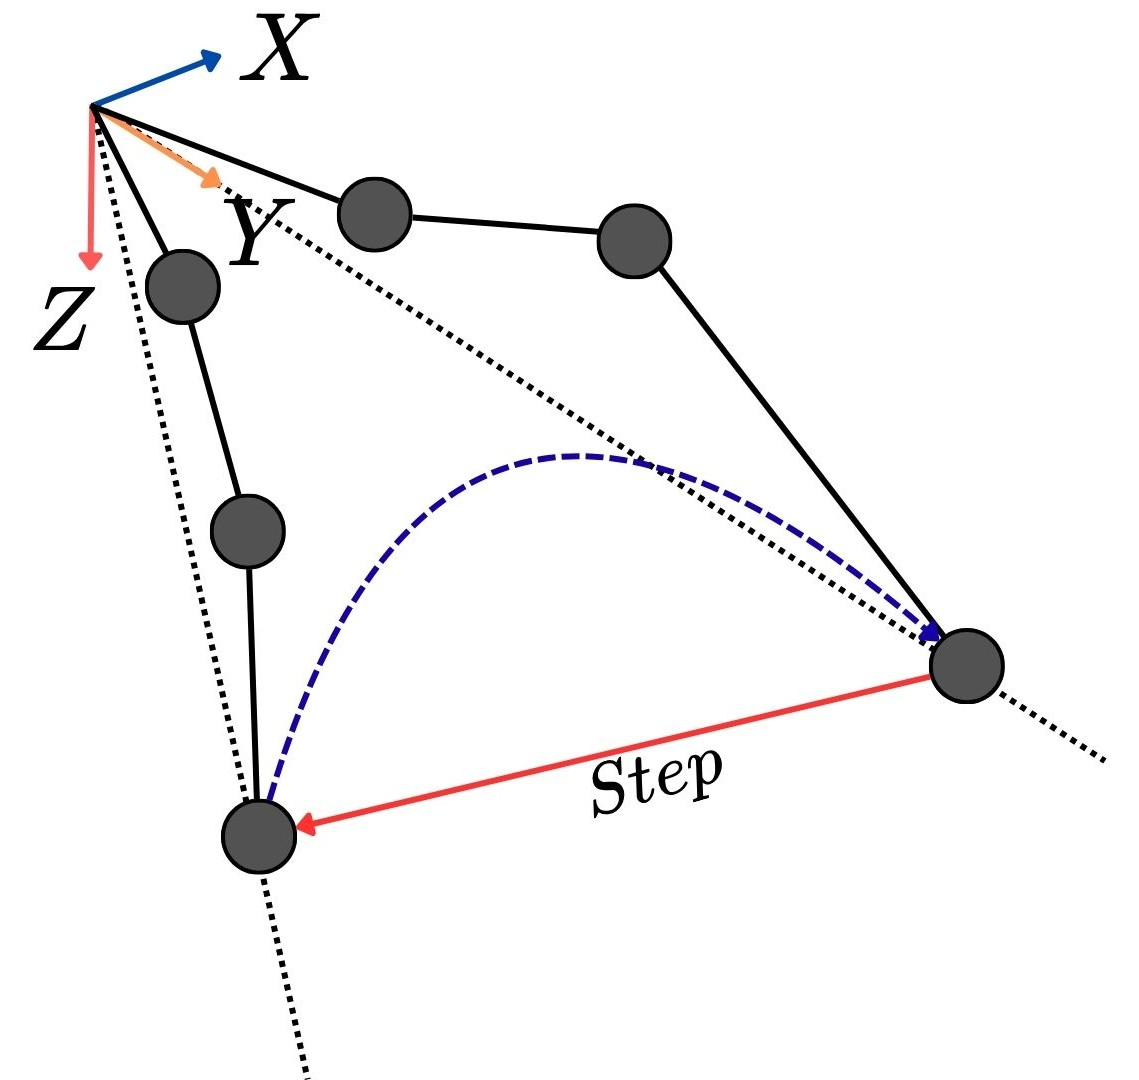
\includegraphics[width=0.9\linewidth]{capitulos/cap2/figuras/swing.jpeg}
        \captionsetup{type=figure,margin=24pt,skip=6pt}
        \captionof{figure}{Trayectoria de la pata en un ciclo de marcha.}
        \label{fig:trayectoria_pata_ciclo}
        \par{\footnotesize Fuente: Elaboración propia.}
    \end{minipage}

    Esta relación establece el vínculo entre la velocidad global del cuerpo y la velocidad local que deben desarrollar las patas durante \textit{swing}. Así, para una marcha muy estable ($\beta=0{,}75$), la velocidad del robot queda limitada aproximadamente a un tercio de la velocidad de retorno de la pata ($V \approx 0{,}33U$), mientras que en marcha trípode ($\beta=0{,}5$) ambas coinciden ($V=U$).
\end{itemize}



\subsection{Patrones de marcha periódica}
\label{subsubsec:gait_patterns}

Dentro de la categoría de marchas periódicas, se han seleccionado tres patrones representativos y recurrentes en la literatura. En conjunto, estos patrones ilustran distintos compromisos entre velocidad, margen de estabilidad y continuidad del apoyo \cite{siciliano2016springer}.

\noindent\textbf{Marcha Trípode (\textit{Tripod Gait}, $\beta = 1/2$):}
Es la marcha periódica estáticamente estable más rápida en un hexápodo. Las patas se organizan en dos trípodes alternos (generalmente \{LT, LB, RM\} y \{RT, RB, LM\}) que operan en contrafase, de modo que mientras un grupo permanece en apoyo el otro ejecuta la fase de transferencia. 

\vspace{-0.7\baselineskip}
\begin{figure}[H]
    \centering

    \begin{minipage}[c]{0.40\textwidth}
        \centering
        \includegraphics[width=\linewidth]{capitulos/cap2/figuras/tripode_poligono.jpeg}
        \vspace{0.2\baselineskip}
        {\footnotesize\textbf{(a)} Polígono de soporte}
    \end{minipage}
    \hfill
    \begin{minipage}[c]{0.55\textwidth}
        \centering
        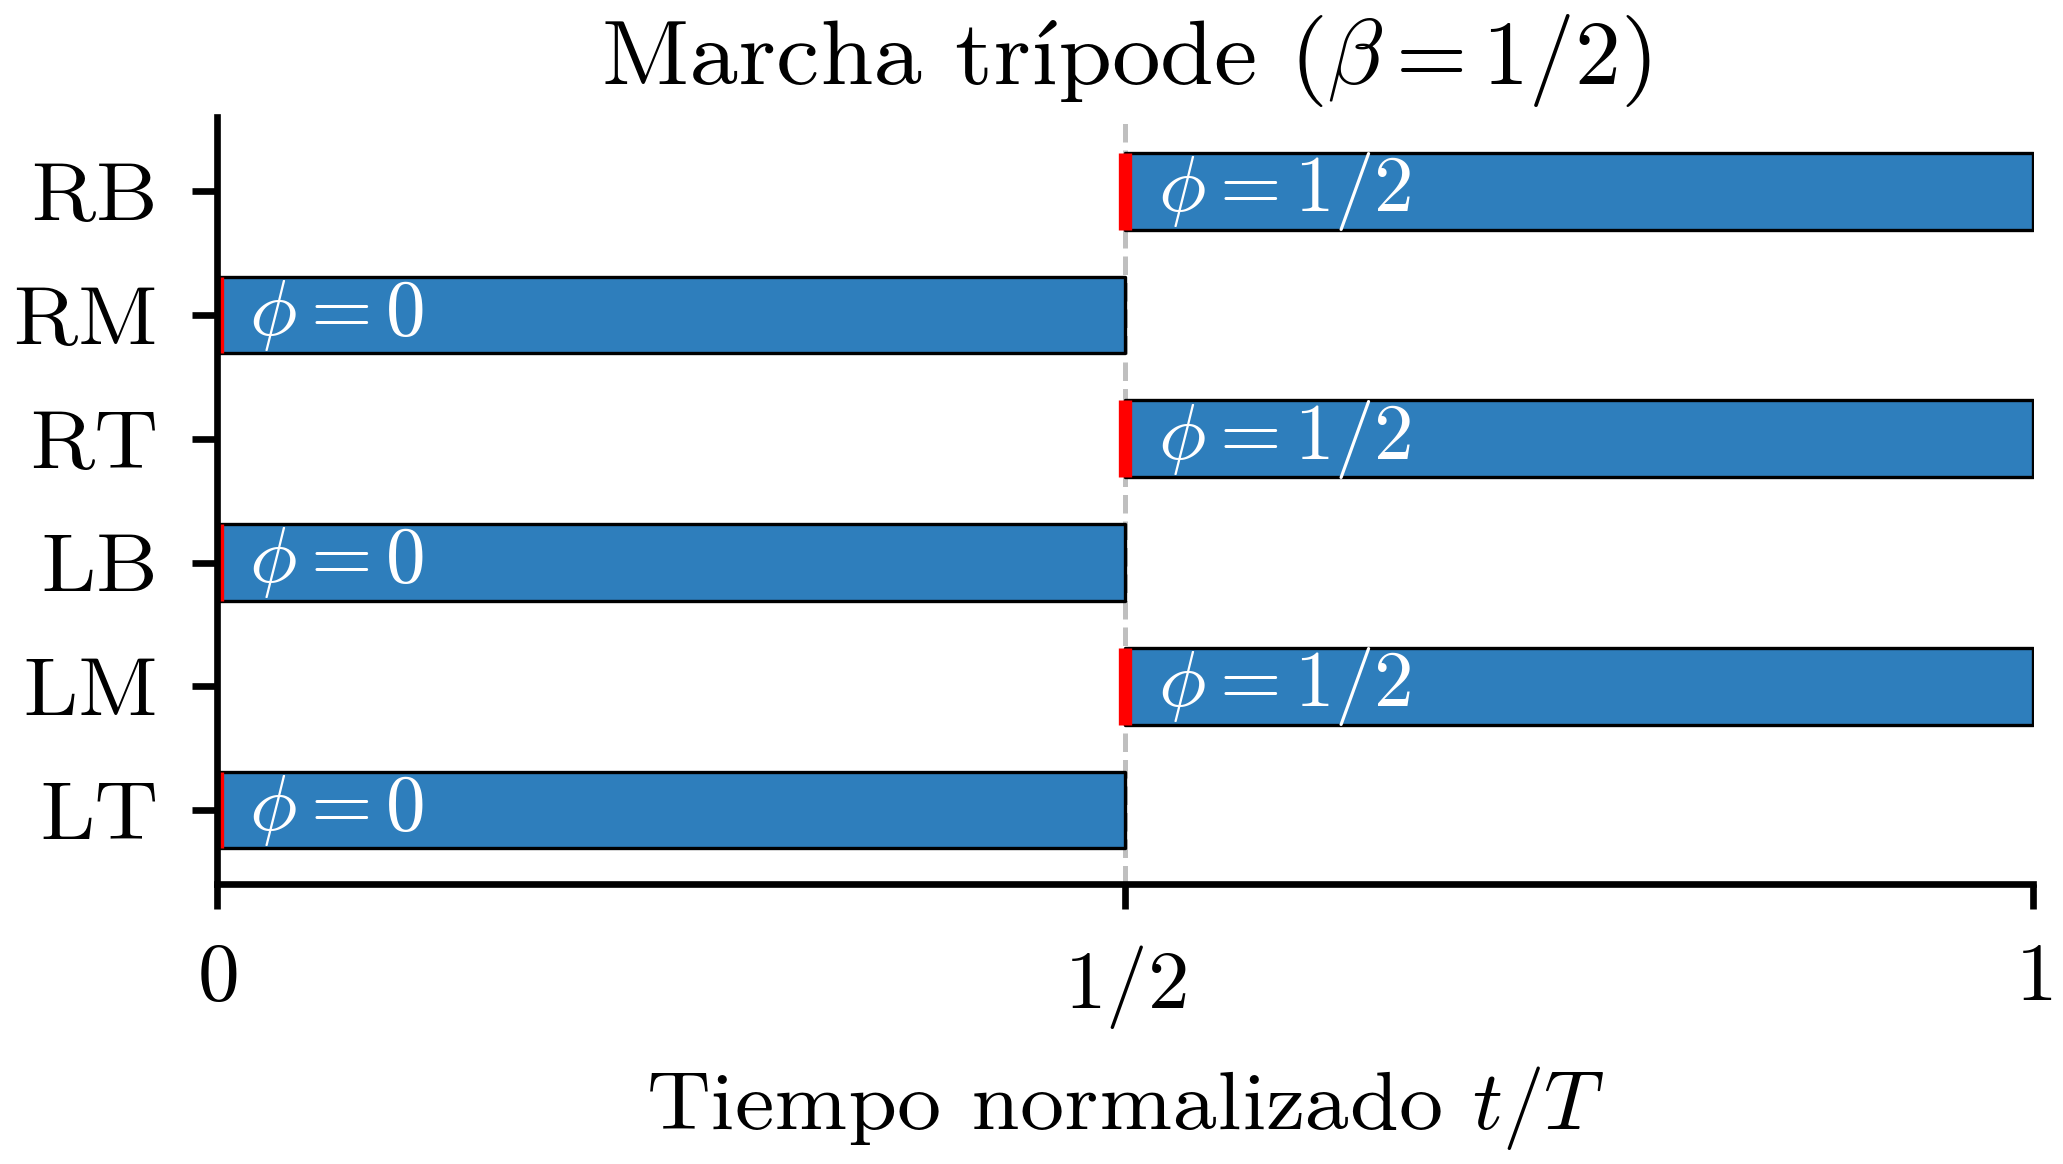
\includegraphics[width=\linewidth]{capitulos/cap2/figuras/tripod_gait.png}
        \vspace{0.2\baselineskip}
        {\footnotesize\textbf{(b)} Diagrama de marcha}
    \end{minipage}

    \captionsetup{justification=centering,skip=4pt}
    \caption[Marcha trípode: polígono y diagrama]{Marcha trípode: (a) polígono de soporte y (b) diagrama de marcha.}
    \label{fig:tripode_poligono_y_diagrama}
    {\footnotesize Fuente: Elaboración propia.}
\end{figure}
\vspace{-1.00\baselineskip}

Como se observa en la Figura~\ref{fig:tripode_poligono_y_diagrama}, al tener un factor de servicio $\beta=0{,}5$, la velocidad de avance del robot iguala a la velocidad de retorno de la pata durante la fase \textit{swing} ($V=U$), según la Ec.~\ref{eq:vel_dynamic}. La marcha trípode mantiene tres apoyos simultáneos y presenta estabilidad estática mientras la proyección del centro de masas permanezca en el interior del triángulo de soporte. Es la marcha con menor margen frente a perturbaciones.

\noindent\textbf{Marcha de Onda (\textit{Wave/Ripple Gait}, $\beta = 5/6$):} En esta configuración, las patas se levantan secuencialmente una a una siguiendo un patrón de ola, de modo que en cualquier instante cinco patas se encuentran en fase de apoyo y solo una en fase de transferencia.

\vspace{-0.7\baselineskip}
\begin{figure}[H]
    \centering

    \begin{minipage}[c]{0.40\textwidth}
        \centering
        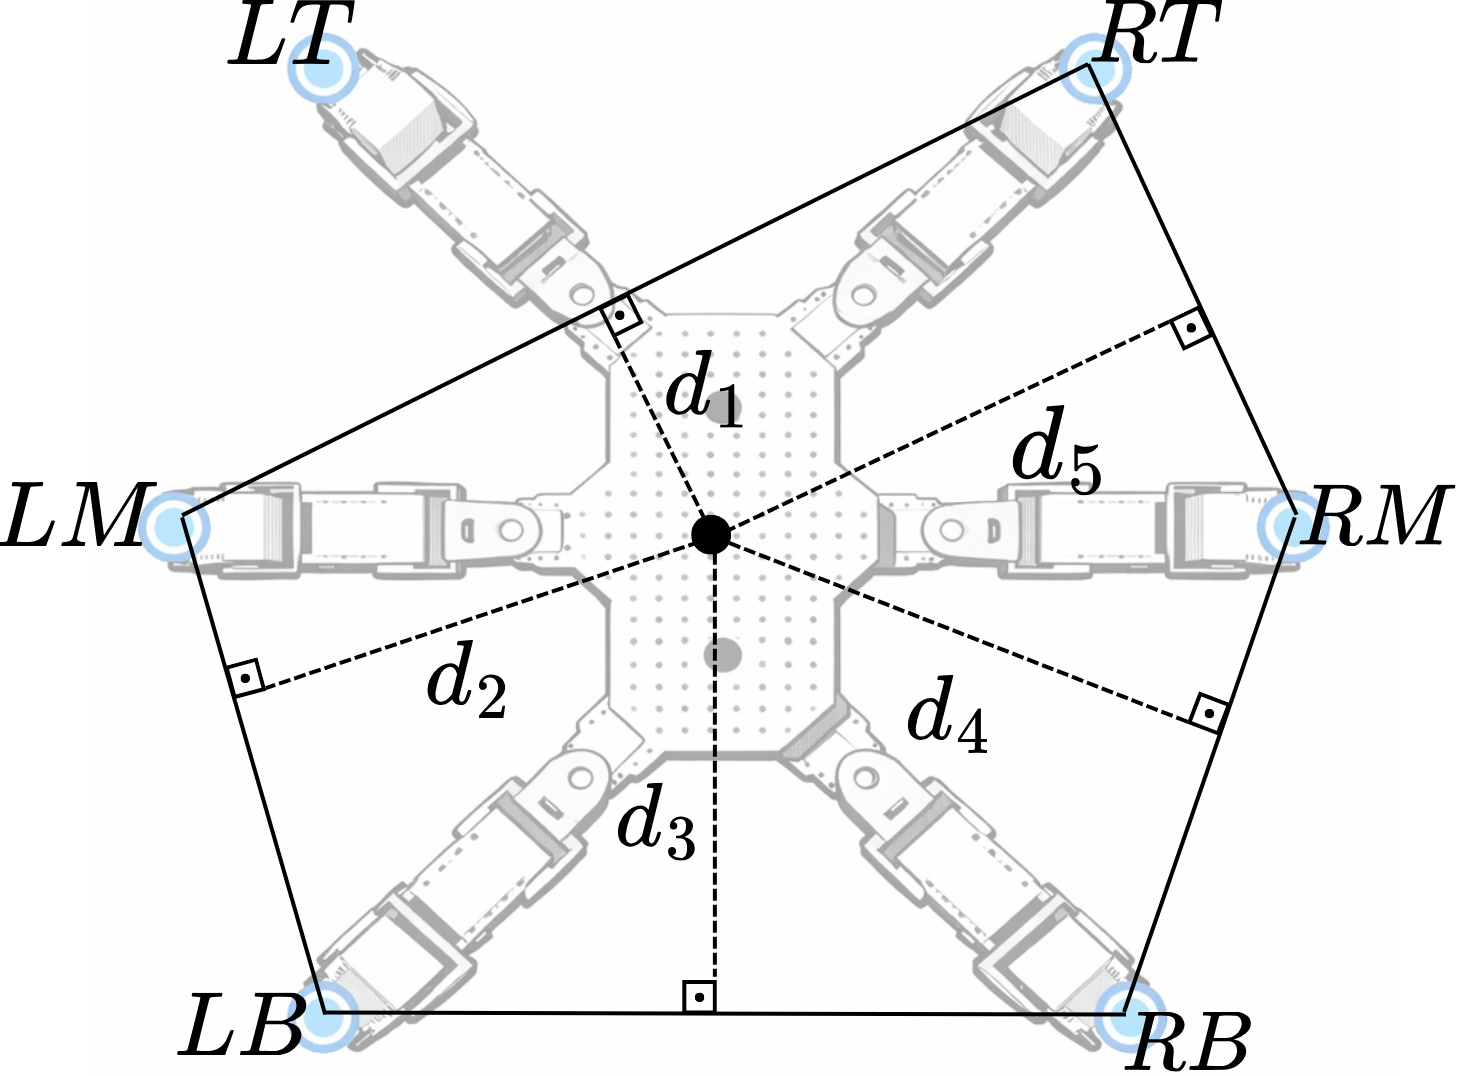
\includegraphics[width=\linewidth]{capitulos/cap2/figuras/Ripple_poligono.jpeg}
        \vspace{0.2\baselineskip}
        {\footnotesize\textbf{(a)} Polígono de soporte.}
    \end{minipage}
    \hfill
    \begin{minipage}[c]{0.55\textwidth}
        \centering
        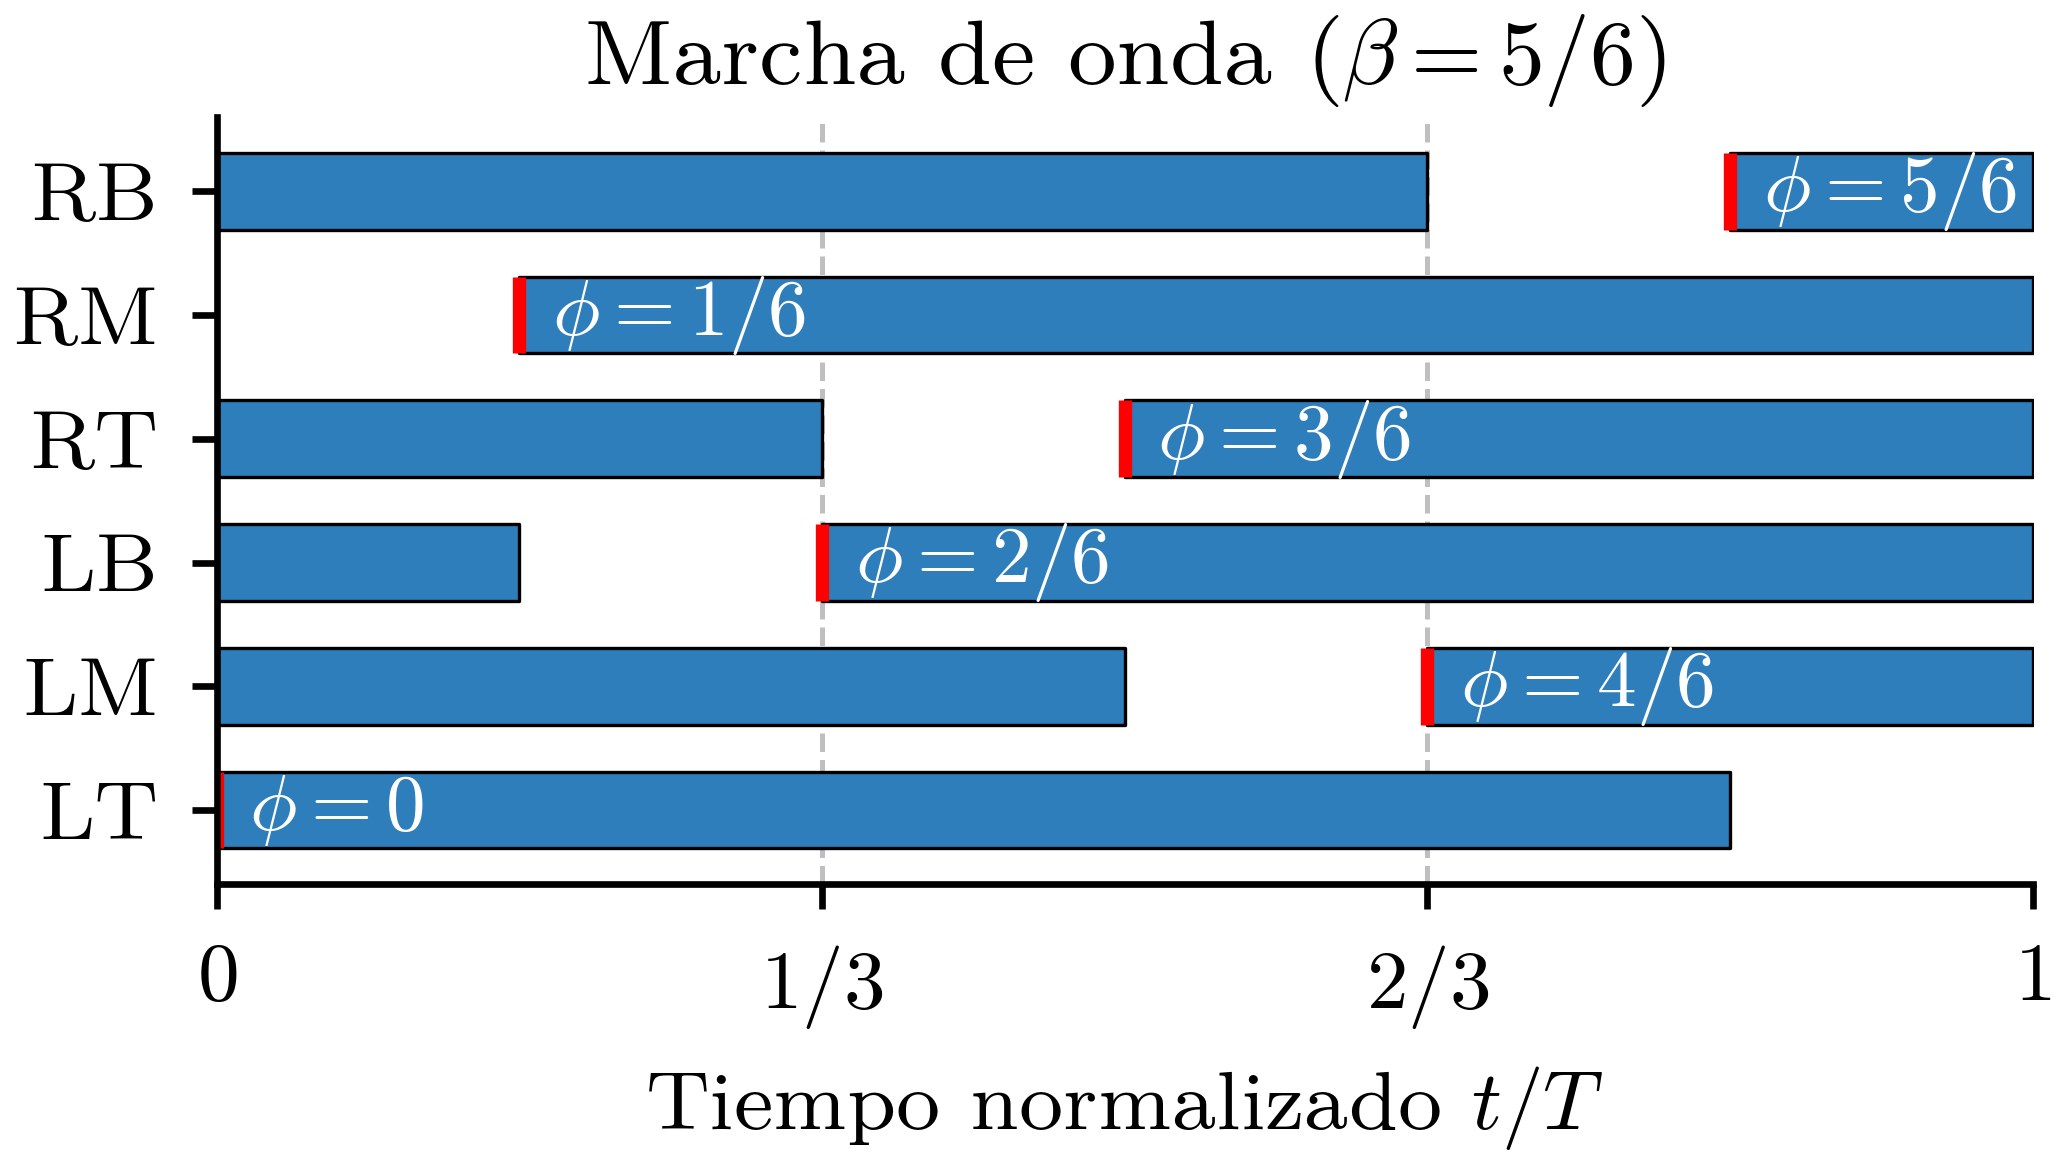
\includegraphics[width=\linewidth]{capitulos/cap2/figuras/ripple_gait.png}
        \vspace{0.2\baselineskip}
        {\footnotesize\textbf{(b)} Diagrama de marcha.}
    \end{minipage}

    \captionsetup{justification=centering,skip=4pt}
    \caption[Marcha de onda: polígono y diagrama]{Marcha de onda: (a) polígono de soporte y (b) diagrama de marcha.}
    \label{fig:ripple_poligono_y_diagrama}
    \footnotesize Fuente: Elaboración propia.
\end{figure}
\vspace{-1.00\baselineskip}

Como muestra la Figura~\ref{fig:ripple_poligono_y_diagrama}, esto da lugar a un polígono de soporte pentagonal, maximizando el margen de estabilidad estática y haciendo esta marcha especialmente adecuada para terrenos irregulares o maniobras de precisión. Como contrapartida, su velocidad teórica es reducida ($V = 0{,}2 \cdot U$).

\par\medskip
\noindent\textbf{Marcha Tetrapódica (\textit{Tetrapod/Amble Gait}, $\beta = 2/3$):}
Representa un compromiso intermedio entre rapidez y estabilidad. Las patas se coordinan por pares, de manera que en régimen periódico permanecen cuatro patas en contacto con el suelo.

\begin{figure}[H]
    \centering

    \begin{minipage}[c]{0.40\textwidth}
        \centering
        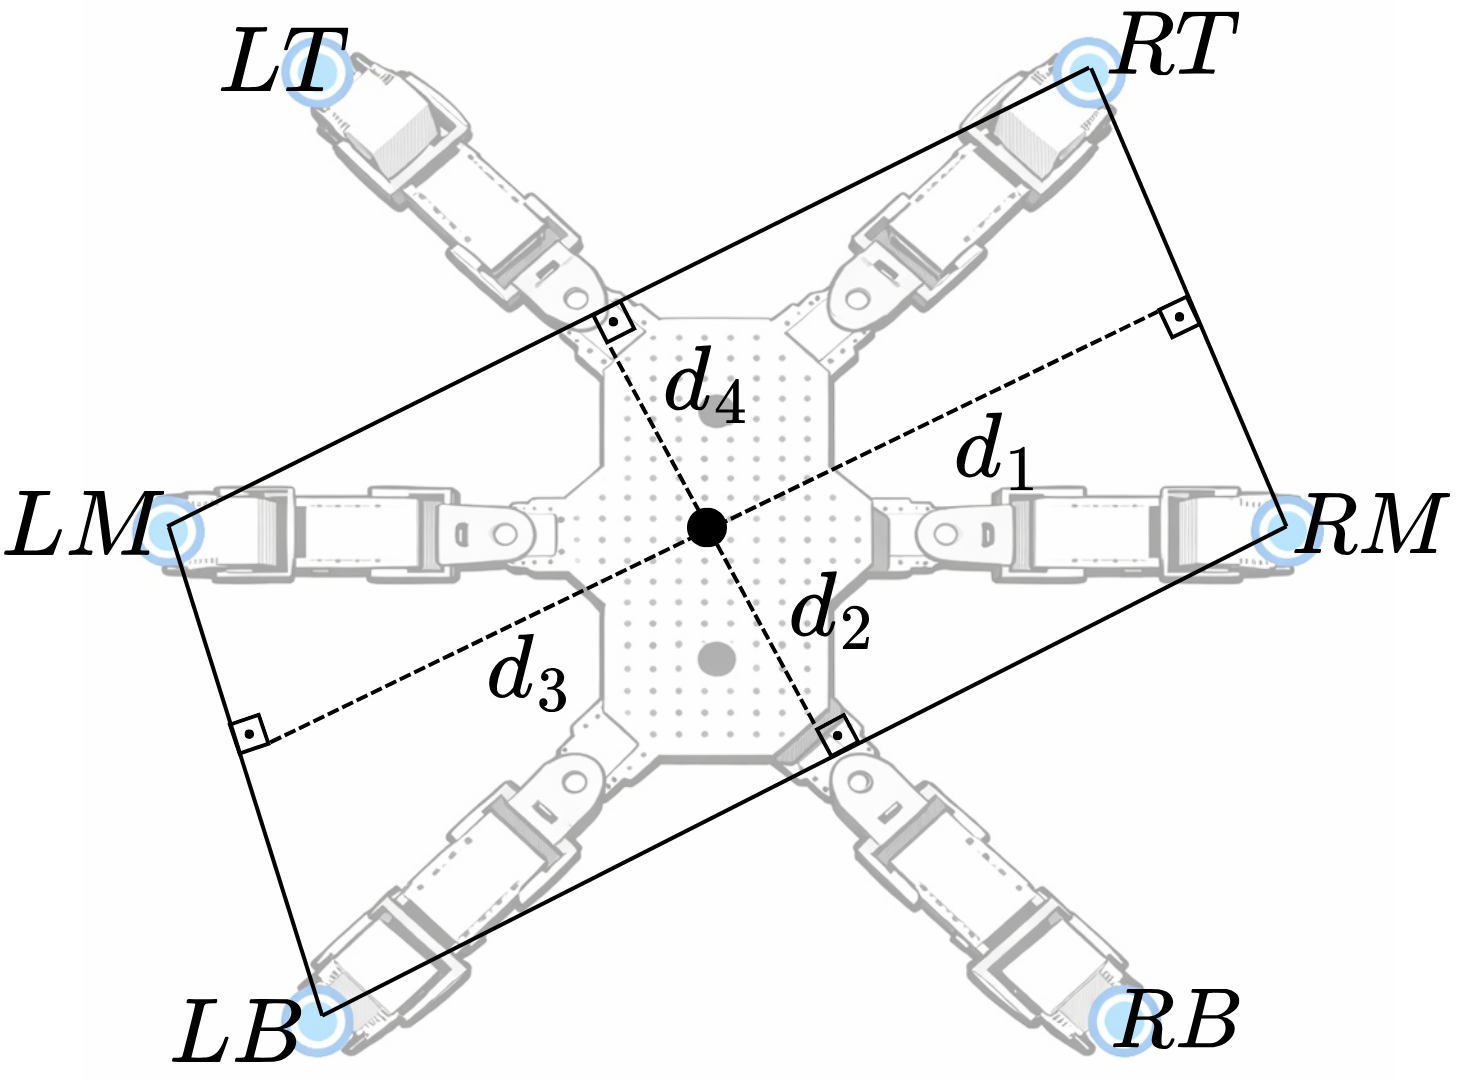
\includegraphics[width=\linewidth]{capitulos/cap2/figuras/tetrapodo_poligono.jpeg}
        \vspace{0.2\baselineskip}
        {\footnotesize\textbf{(a)} Polígono de soporte.}
    \end{minipage}
    \hfill
    \begin{minipage}[c]{0.55\textwidth}
        \centering
        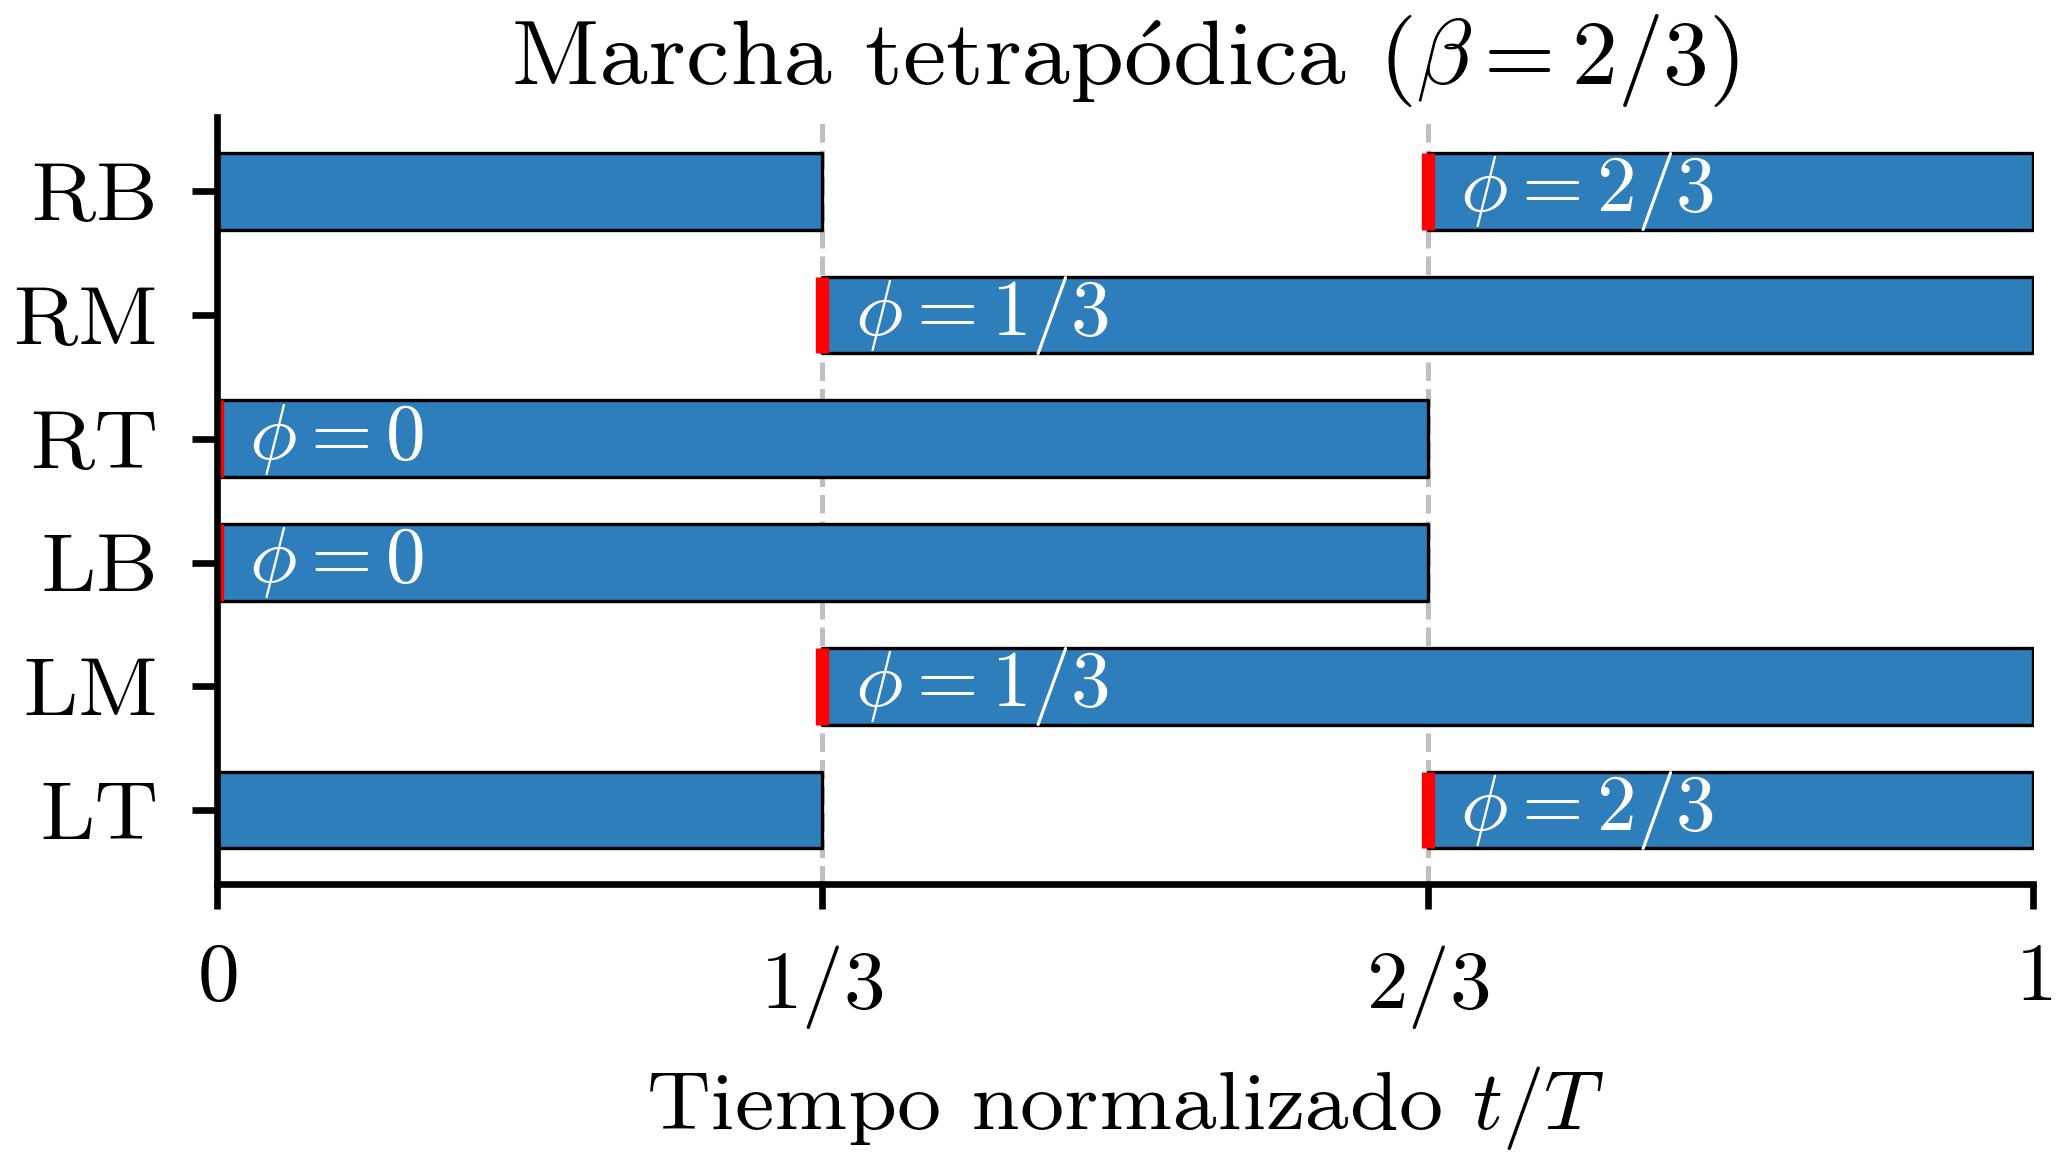
\includegraphics[width=\linewidth]{capitulos/cap2/figuras/amble_gait.png}
        \vspace{0.2\baselineskip}
        {\footnotesize\textbf{(b)} Diagrama de marcha}
    \end{minipage}

    \captionsetup{justification=centering}
    \caption[Marcha tetrapódica: polígono y diagrama]{Marcha tetrapódica: (a) polígono de soporte y (b) diagrama de marcha.}
    \label{fig:tetrapodo_poligono}
    {\footnotesize Fuente: Elaboración propia.}
\end{figure}
\vspace{-1.00\baselineskip}

Como se aprecia en la Figura~\ref{fig:tetrapodo_poligono}, con un factor de servicio de $\beta \approx 0{,}67$, ofrece mayor estabilidad que la marcha trípode y mayor velocidad que la marcha de onda ($V = 0{,}5 \cdot U$), proporcionando una redundancia de apoyo útil cuando la tracción del suelo no es perfecta.

\section{Planificación de trayectorias}
\label{subsec:trajectory_planning}

La generación de movimiento en el hexápodo requiere definir la evolución temporal de las coordenadas, ya que aplicar cambios instantáneos a los servomotores provocaría aceleraciones teóricamente infinitas. Una vez fijado el patrón temporal de la marcha, el siguiente problema consiste en determinar cómo evoluciona espacialmente cada pata.

\vspace{-0.5\baselineskip}
\subsection{Perfil de trayectoria de vuelo (swing phase)}
\label{subsec:theory_swing}

La trayectoria de la pata se parametriza mediante una fase normalizada $u\in[0,1]$, donde $u=0$ corresponde al instante de despegue y $u=1$ al de aterrizaje. Bajo esta variable, la planificación se desacopla en una componente vertical, que garantiza el despeje respecto al suelo, y una componente horizontal, que recoloca la pata en el siguiente punto de apoyo.

\vspace{-0.5\baselineskip}
\paragraph{Elevación vertical ($Z$):}
El término $\Delta z_{step}(u)$ introducido en la componente vertical de la Ec.~\ref{eq:swing_global_calc} se modela mediante un perfil sinusoidal cuadrático. Esta elección conserva la sencillez geométrica de una ley senoidal y, al mismo tiempo, proporciona un comportamiento suave en los instantes de despegue y aterrizaje:

\vspace{-1\baselineskip}
\begin{equation}
    \Delta z_{step}(u) = H_{step}\,\sin^2(\pi u)
    \label{eq:swing_profile_z}
\end{equation}
\vspace{-1.5\baselineskip}

Con esta expresión se satisfacen las condiciones geométricas deseadas para la fase de elevación: $\Delta z_{step}(0)=0$ y $\Delta z_{step}(1)=0$, de modo que el pie despega desde la cota de referencia y vuelve a ella al finalizar el \textit{swing}. Además, $\Delta z_{step}\!\left(\frac{1}{2}\right)=H_{step}$, por lo que la altura máxima se alcanza en el punto medio del recorrido. Para estudiar la suavidad del perfil, se deriva respecto a la variable normalizada $u$:

\vspace{-0.5\baselineskip}
\begin{equation}
    \frac{d\,\Delta z_{step}}{du}
    =
    2\pi H_{step}\sin(\pi u)\cos(\pi u)
    =
    \pi H_{step}\sin(2\pi u)
    \label{eq:swing_profile_z_du}
\end{equation}
\vspace{-1\baselineskip}

De la Ec.~\ref{eq:swing_profile_z_du} se deduce que los puntos críticos aparecen en $u=0$, $u=\frac{1}{2}$ y $u=1$. En particular, evaluando la derivada en los extremos:
\begin{equation}
    \left.\frac{d\,\Delta z_{step}}{du}\right|_{u=0}
    =
    \left.\frac{d\,\Delta z_{step}}{du}\right|_{u=1}
    =0
    \label{eq:swing_profile_z_zero_slope}
\end{equation}
\vspace{-1\baselineskip}

por lo que la trayectoria presenta pendiente nula tanto al inicio como al final de la fase de vuelo. Esto implica que el pie inicia y finaliza la elevación sin cambios bruscos en la componente vertical, lo que se traduce en un movimiento más suave y controlado, como se observa en la Figura~\ref{fig:sin2_vertical_profiles}. 

\begin{figure}[H]
    \centering
    \begin{minipage}[t]{0.45\textwidth}
        \centering
        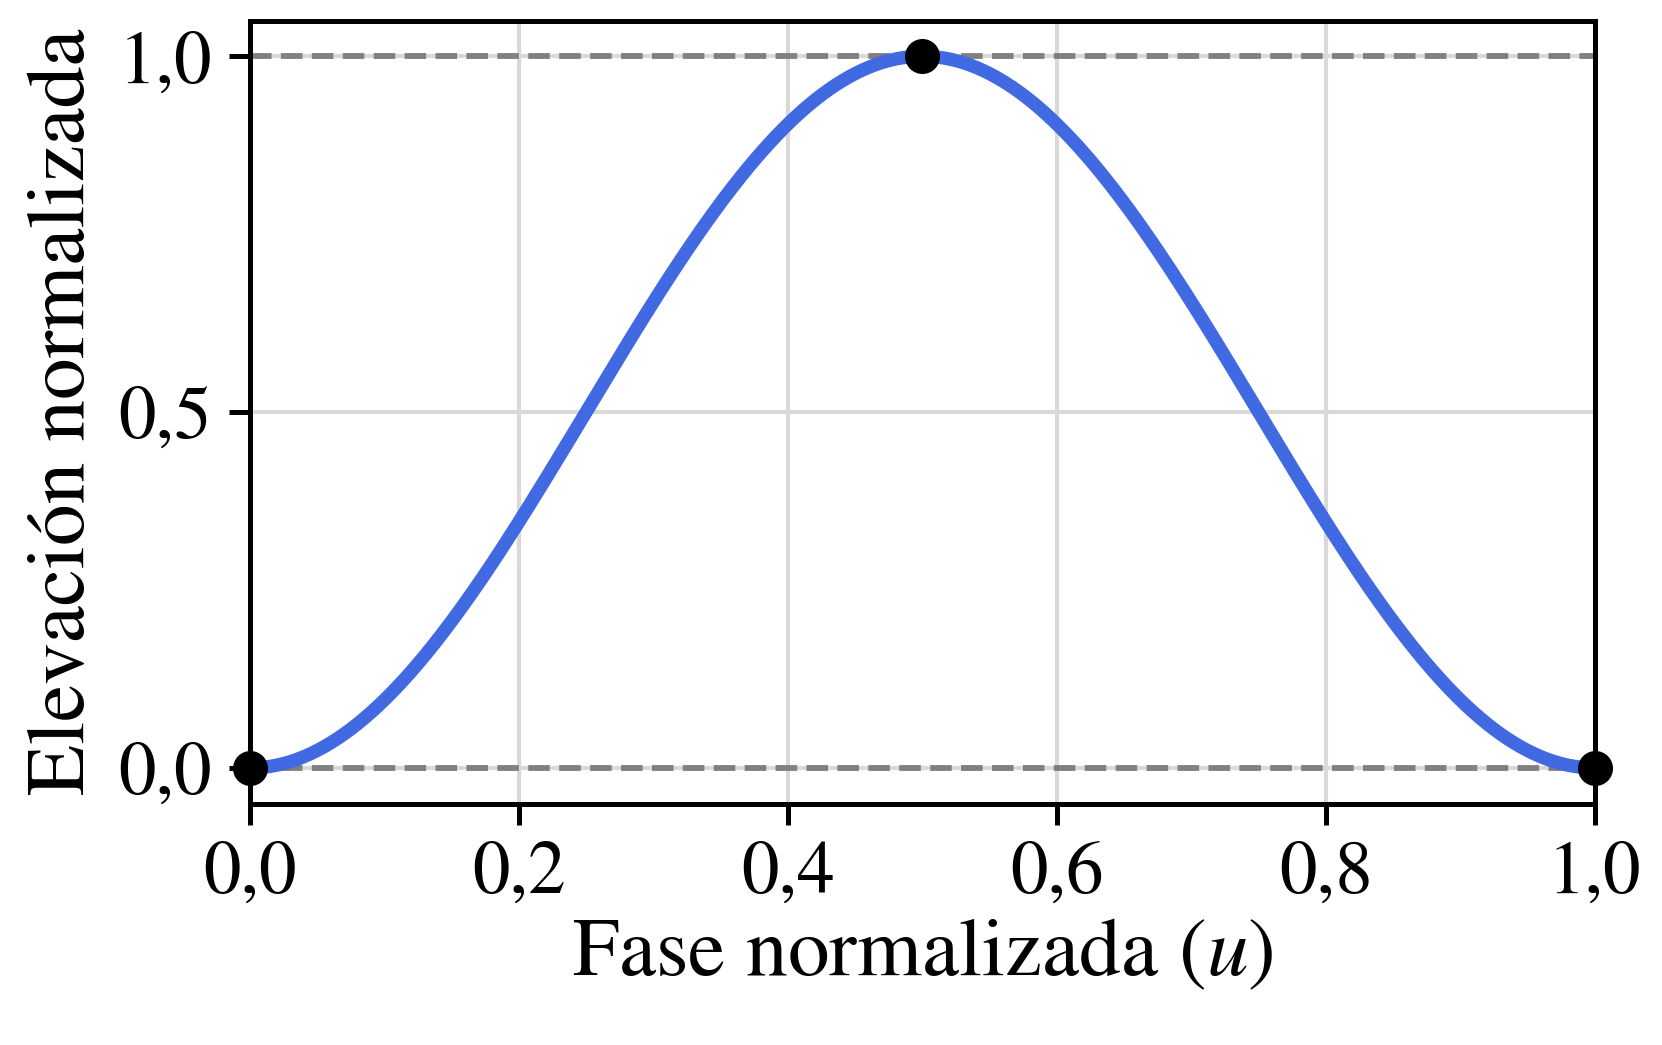
\includegraphics[width=\linewidth]{capitulos/cap2/figuras/sin2_vertical_pos.png}

        \vspace{0.05em}
        {\footnotesize (a) $\Delta z_{step}(u)/H_{step}=\sin^2(\pi u)$.}
    \end{minipage}
    \hspace{0.04\textwidth}
    \begin{minipage}[t]{0.45\textwidth}
        \centering
        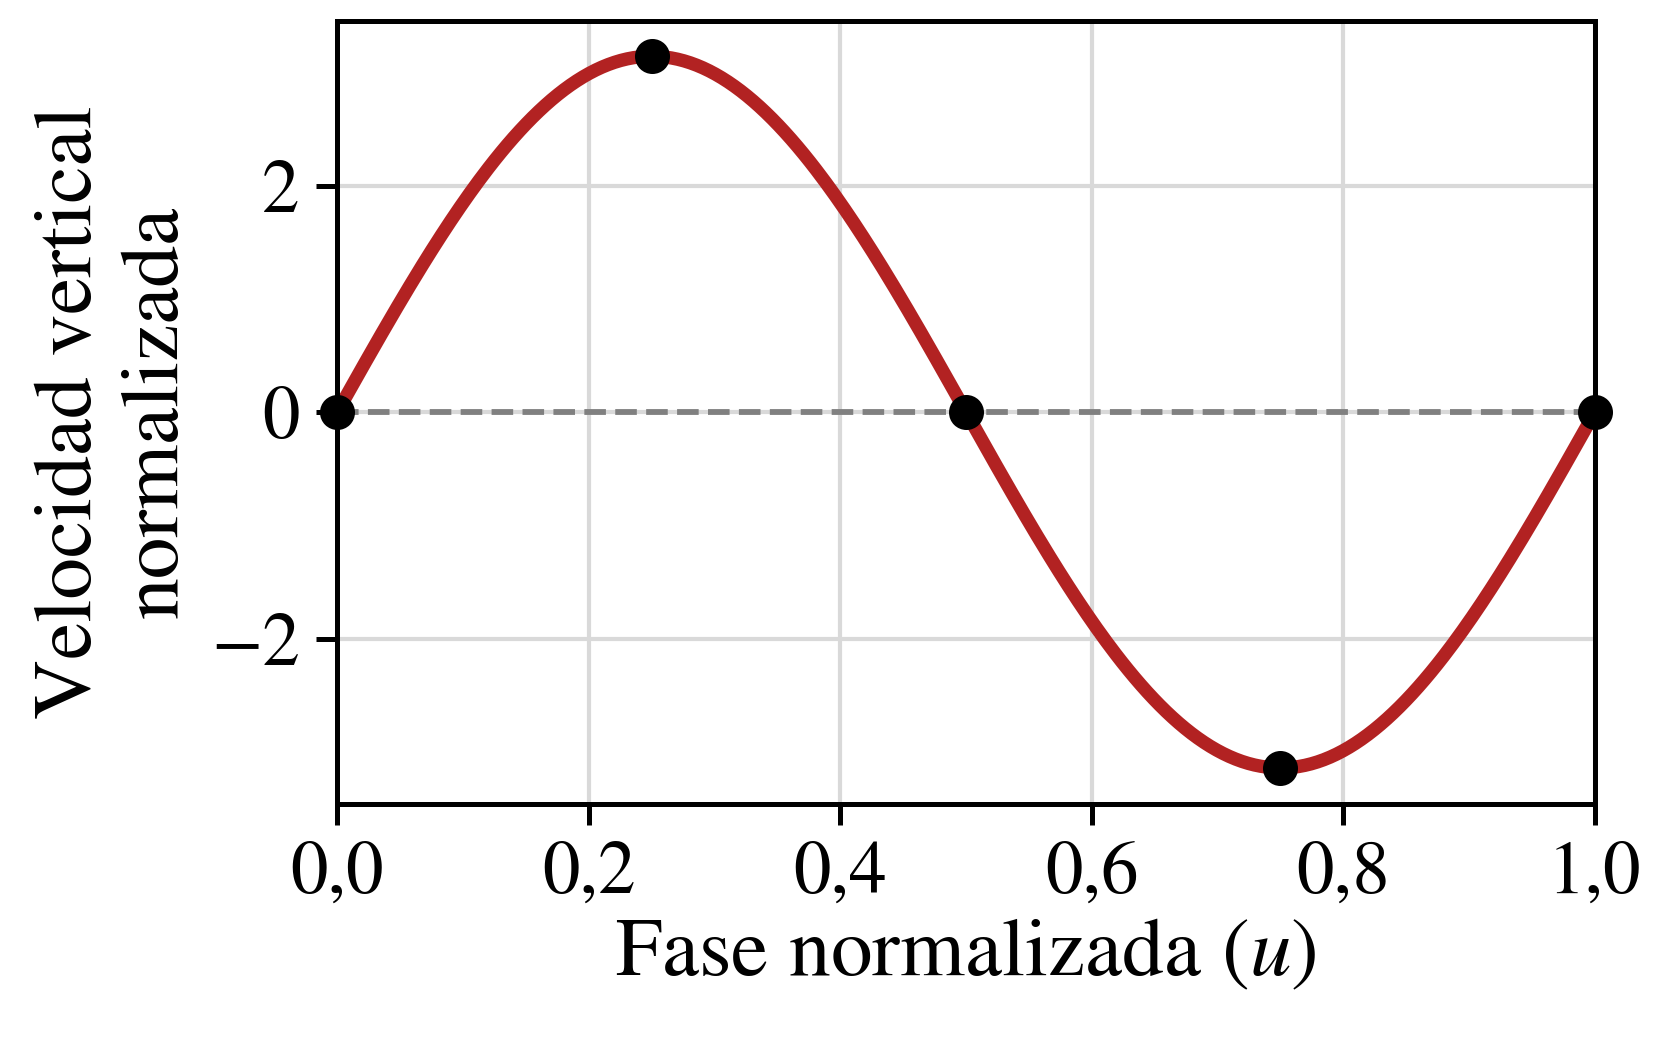
\includegraphics[width=\linewidth]{capitulos/cap2/figuras/sin2_vertical_vel.png}

        \vspace{0.05em}
        {\footnotesize (b) $\frac{1}{H_{step}}\frac{d\,\Delta z_{step}}{du}=\pi\sin(2\pi u)$.}
    \end{minipage}

    \captionsetup{skip=1pt,justification=centering}
    \caption[Perfil vertical sinusoidal cuadrático]{Perfil vertical sinusoidal cuadrático: evolución de la posición y de la velocidad normalizadas durante la fase de \textit{swing}.}
    \label{fig:sin2_vertical_profiles}
    \par{\footnotesize Fuente: Elaboración propia mediante
    MATLAB~\cite{matlab}.}
\end{figure}

\vspace{-1\baselineskip}
\paragraph{Avance horizontal ($XY$):}
El desplazamiento en el plano, encargado de recolocar la pata en el siguiente punto de apoyo, se modela mediante una interpolación polinómica cúbica sobre esta misma fase normalizada $u$. Esta elección permite imponer de forma directa las condiciones de contorno del movimiento y, al mismo tiempo, garantiza que la pata inicie y finalice el \textit{swing} sin velocidades horizontales bruscas. Para ello, se parte del polinomio general:

\vspace{-1.5\baselineskip}
\setlength{\abovedisplayskip}{0pt}
\setlength{\abovedisplayshortskip}{0pt}
\begin{equation}
    f(u) = c_3u^3 + c_2u^2 + c_1u + c_0
    \label{eq:smoothstep_poly_general}
\end{equation}
\vspace{-1\baselineskip}

Sobre este polinomio se imponen las condiciones geométricas deseadas para la fase de avance: el pie debe recorrer el paso completo, $f(0)=0$ y $f(1)=1$, partiendo y llegando con velocidad nula, $f'(0)=f'(1)=0$. Estas restricciones se resumen en la Ec.~\ref{eq:boundary_conditions}. Al aplicarlas en $u=0$ se obtiene directamente $c_0=c_1=0$, mientras que las restantes conducen al sistema de la Ec.~\ref{eq:smoothstep_system}, cuya solución es $c_2=3$ y $c_3=-2$.
\vspace{-1\baselineskip}

\noindent
\begin{minipage}[t]{0.48\textwidth}
    \begin{equation}
    \begin{cases}
        f(0) = 0, \quad f(1) = 1 \\
        f'(0) = 0, \quad f'(1) = 0
    \end{cases}
    \label{eq:boundary_conditions}
\end{equation}
    \end{minipage}
\hfill
\begin{minipage}[t]{0.48\textwidth}
    \begin{equation}
    \begin{cases}
        c_3 + c_2 = 1 \\
        3c_3 + 2c_2 = 0
    \end{cases}
    \label{eq:smoothstep_system}
\end{equation}
    \end{minipage}

Sustituyendo estos valores, se obtiene finalmente la ley de interpolación horizontal:

\vspace{-1.0\baselineskip}
\begin{equation}
    f_{xy}(u) = 3u^2 - 2u^3
    \label{eq:smoothstep_xy_derived}
\end{equation}
\vspace{-1.0\baselineskip}

En este caso, la suavidad en los extremos no requiere verificación adicional, puesto que la velocidad nula en el despegue y el aterrizaje forma parte de las condiciones impuestas en la Ec.~\ref{eq:boundary_conditions}, tal como se aprecia en la Figura~\ref{fig:smoothstep_xy_profiles}.

\begin{figure}[H]
    \centering
    \begin{minipage}[t]{0.495\textwidth}
        \centering
        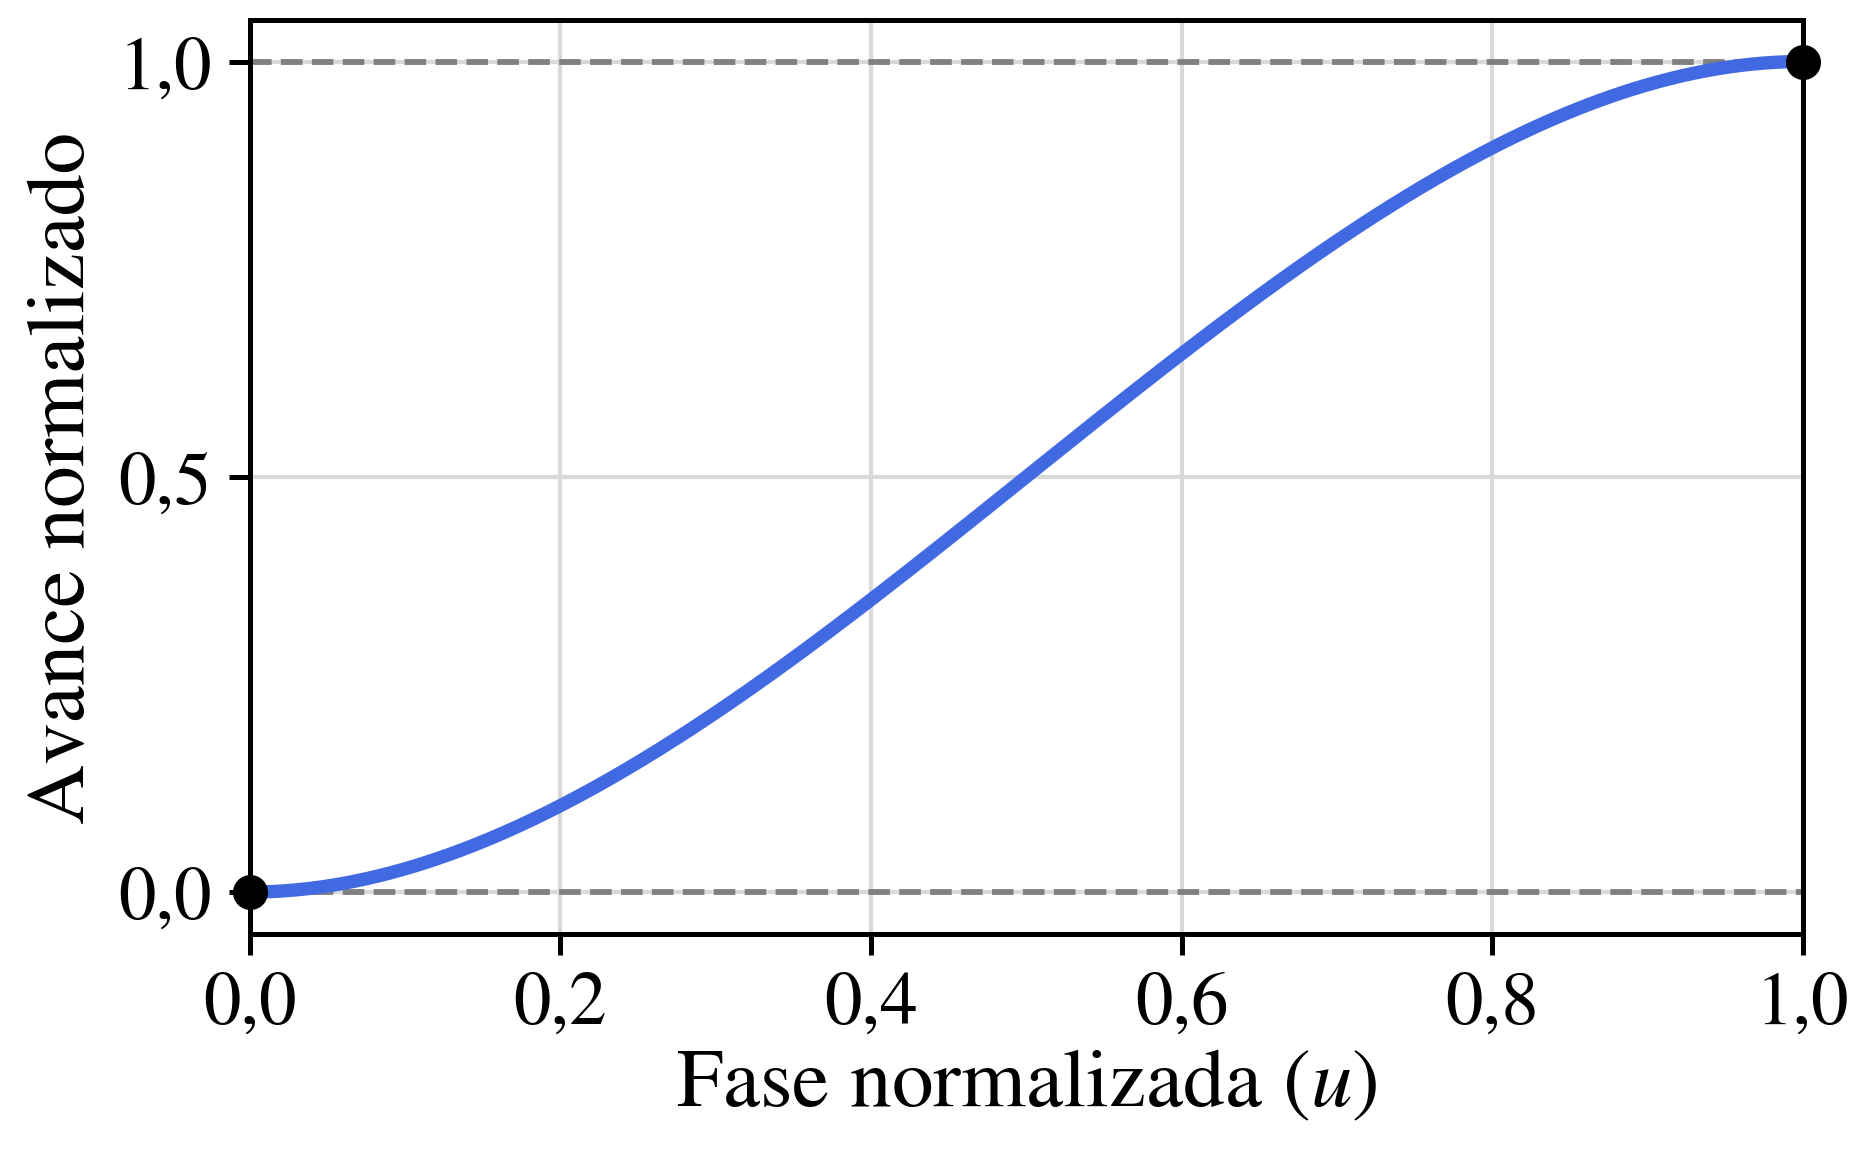
\includegraphics[width=\linewidth]{capitulos/cap2/figuras/3cubic.png}

        \vspace{0.15em}
        {\footnotesize (a) $f_{xy}(u)=3u^2-2u^3$.}
    \end{minipage}
    \hfill
    \begin{minipage}[t]{0.495\textwidth}
        \centering
        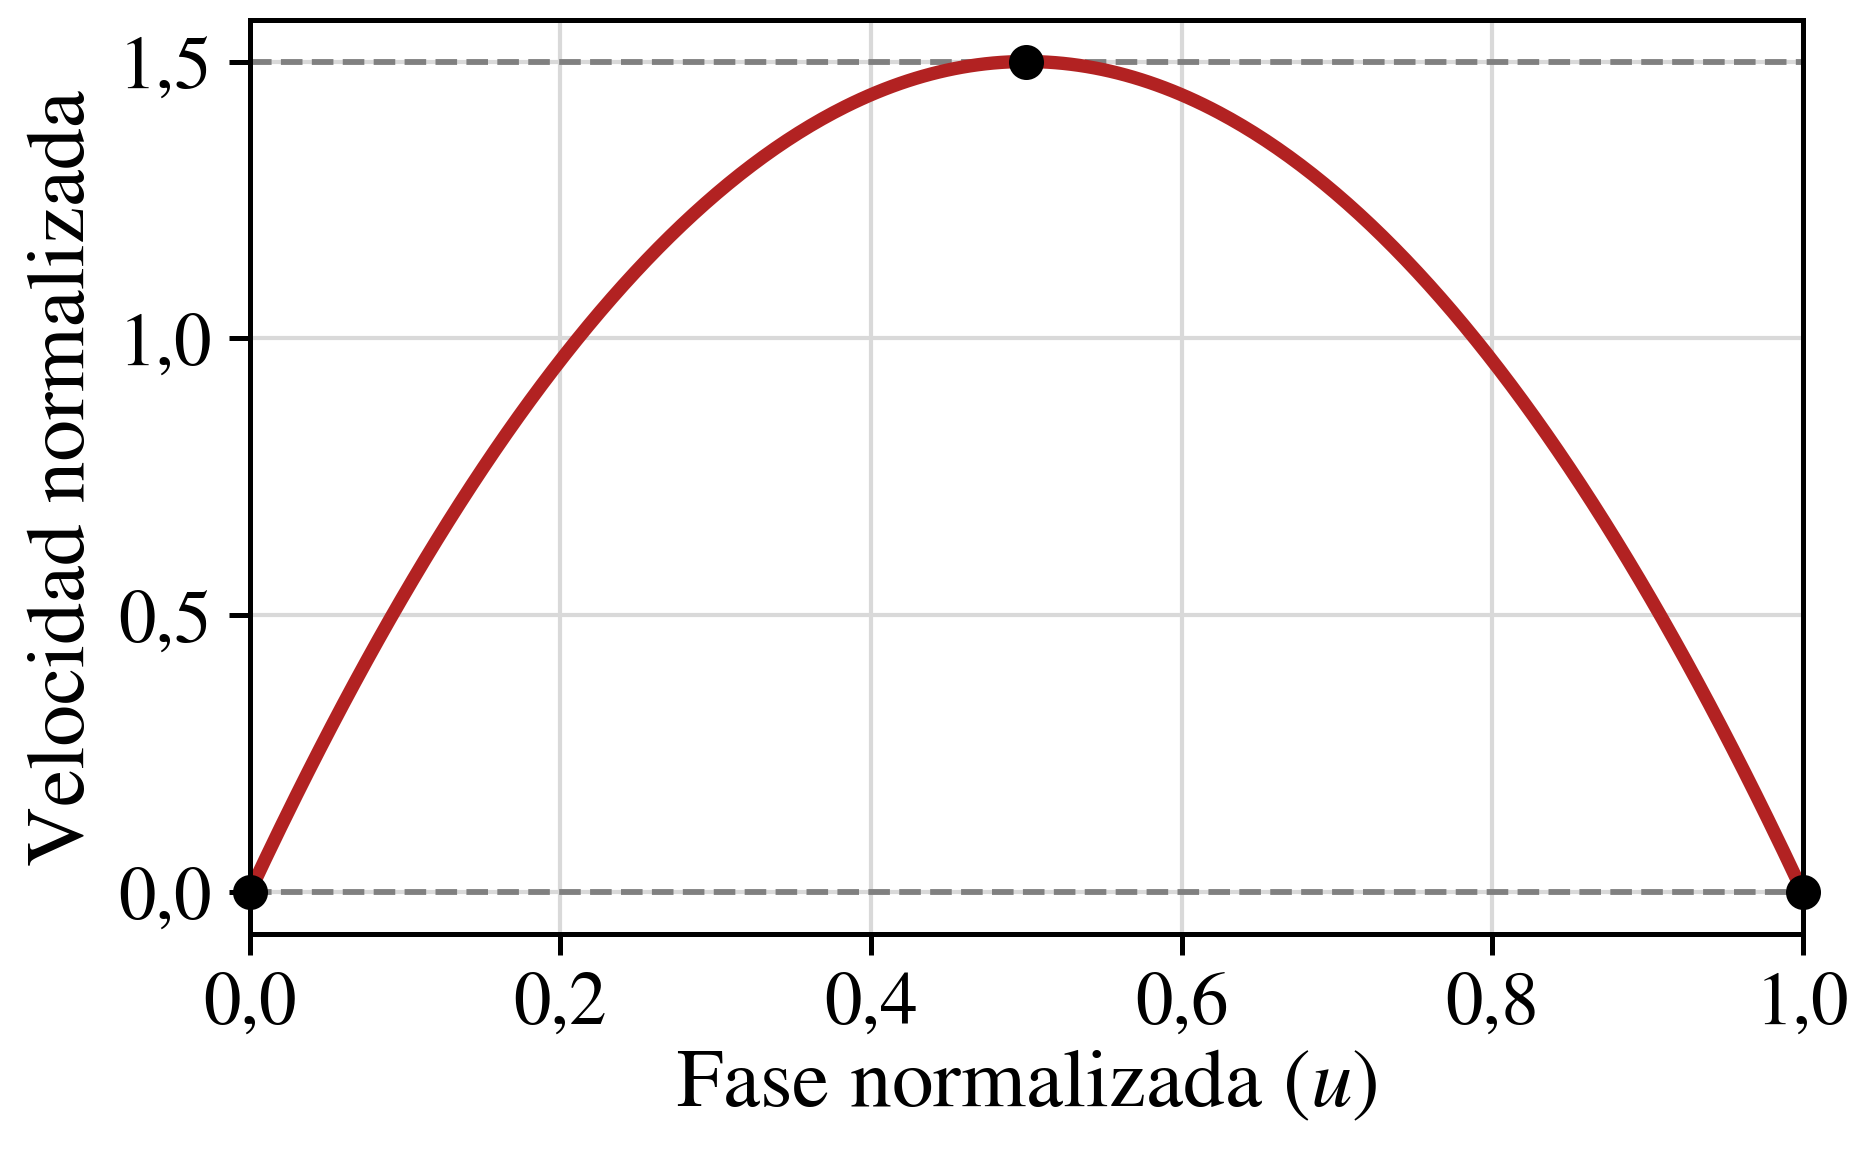
\includegraphics[width=\linewidth]{capitulos/cap2/figuras/3cubic_deriv.png}

        \vspace{0.15em}
        {\footnotesize (b) $\frac{d\,f_{xy}}{du}=6u(1-u)$.}
    \end{minipage}

    \captionsetup{skip=3pt,justification=centering}
    \caption[Perfil horizontal cúbico]{Perfil horizontal cúbico: evolución de la posición y de la velocidad normalizadas durante la fase de \textit{swing}.}
    \label{fig:smoothstep_xy_profiles}
    \par{\footnotesize Fuente: Elaboración propia mediante
    MATLAB~\cite{matlab}.}
\end{figure}
\vspace{-1\baselineskip}

En el caso nominal de paso constante, sin giro y con postura local nula,
esta ley puede escribirse en su forma
centrada:

\vspace{-0.5\baselineskip}
\begin{equation}
    a(u)=f_{xy}(u)-\frac{1}{2}
    \label{eq:smoothstep_centered}
\end{equation}

Con ello, la trayectoria horizontal queda referida a la postura neutral y el
pie recorre simétricamente el intervalo
$\left[{}^{B}{\bm{p}}_{neu}-\bm{s}_{step}/2,\;
{}^{B}{\bm{p}}_{neu}+\bm{s}_{step}/2\right]$. Esta forma centrada es
algebraicamente equivalente a la interpolación de la Ec.~\ref{eq:swing_latched_interp} cuando
los extremos coinciden con los nominales.

\subsection{Suavizado de postura}
\label{subsec:theory_posture_smoothing}

Para las transiciones de postura del cuerpo (cambios de altura, inclinación o rotación), se requiere una suavidad superior a la de la trayectoria de la pata. Mientras que el perfil cúbico garantiza velocidad nula en los extremos, permite saltos instantáneos en la aceleración, lo que puede inducir vibraciones estructurales. Para mitigar esto, se implementa un interpolador de quinto orden \cite{craig2018robotics}. Para ello, se parte del polinomio general:

\vspace{-1\baselineskip}
\setlength{\abovedisplayskip}{0pt}
\setlength{\abovedisplayshortskip}{0pt}
\begin{equation}
    S(t) = c_5t^5 + c_4t^4 + c_3t^3 + c_2t^2 + c_1t + c_0
    \label{eq:quintic_poly_general}
\end{equation}
\vspace{-1.5\baselineskip}

Sobre este polinomio se imponen seis condiciones de contorno: el perfil debe recorrer la transición completa, $S(0)=0$ y $S(1)=1$, con velocidad y aceleración nulas en ambos extremos, $S'(0)=S'(1)=0$ y $S''(0)=S''(1)=0$. Estas restricciones se resumen en la Ec.~\ref{eq:quintic_boundary}. Al aplicarlas en $t=0$ se obtiene directamente $c_0=c_1=c_2=0$, mientras que las restantes conducen al sistema de la Ec.~\ref{eq:quintic_system}, cuya solución es $c_3=10$, $c_4=-15$ y $c_5=6$.

\vspace{-1\baselineskip}
\noindent
\begin{minipage}[t]{0.55\textwidth}
    \begin{equation}
    \begin{cases}
        S(0) = 0, \quad S(1) = 1 \\
        S'(0) = 0, \quad S'(1) = 0 \\
        S''(0) = 0, \quad S''(1) = 0
    \end{cases}
    \label{eq:quintic_boundary}
\end{equation}
    \end{minipage}
\hfill
\begin{minipage}[t]{0.43\textwidth}
    \begin{equation}
    \begin{cases}
        c_5 + c_4 + c_3 = 1 \\
        5c_5 + 4c_4 + 3c_3 = 0 \\
        20c_5 + 12c_4 + 6c_3 = 0
    \end{cases}
    \label{eq:quintic_system}
\end{equation}
    \end{minipage}

Sustituyendo estos valores, se obtiene finalmente la función de mezcla de quinto orden:

\vspace{-1\baselineskip}
\begin{equation}
    S(t) = 6t^5 - 15t^4 + 10t^3
    \label{eq:smootherstep_poly}
\end{equation}
\vspace{-1.5\baselineskip}

La suavidad queda de nuevo garantizada por construcción, con la diferencia de que ahora también la aceleración se anula en los extremos, tal como se aprecia en la Figura~\ref{fig:quintic_profiles}.

\noindent
\begin{minipage}[t]{0.47\textwidth}
    \centering
    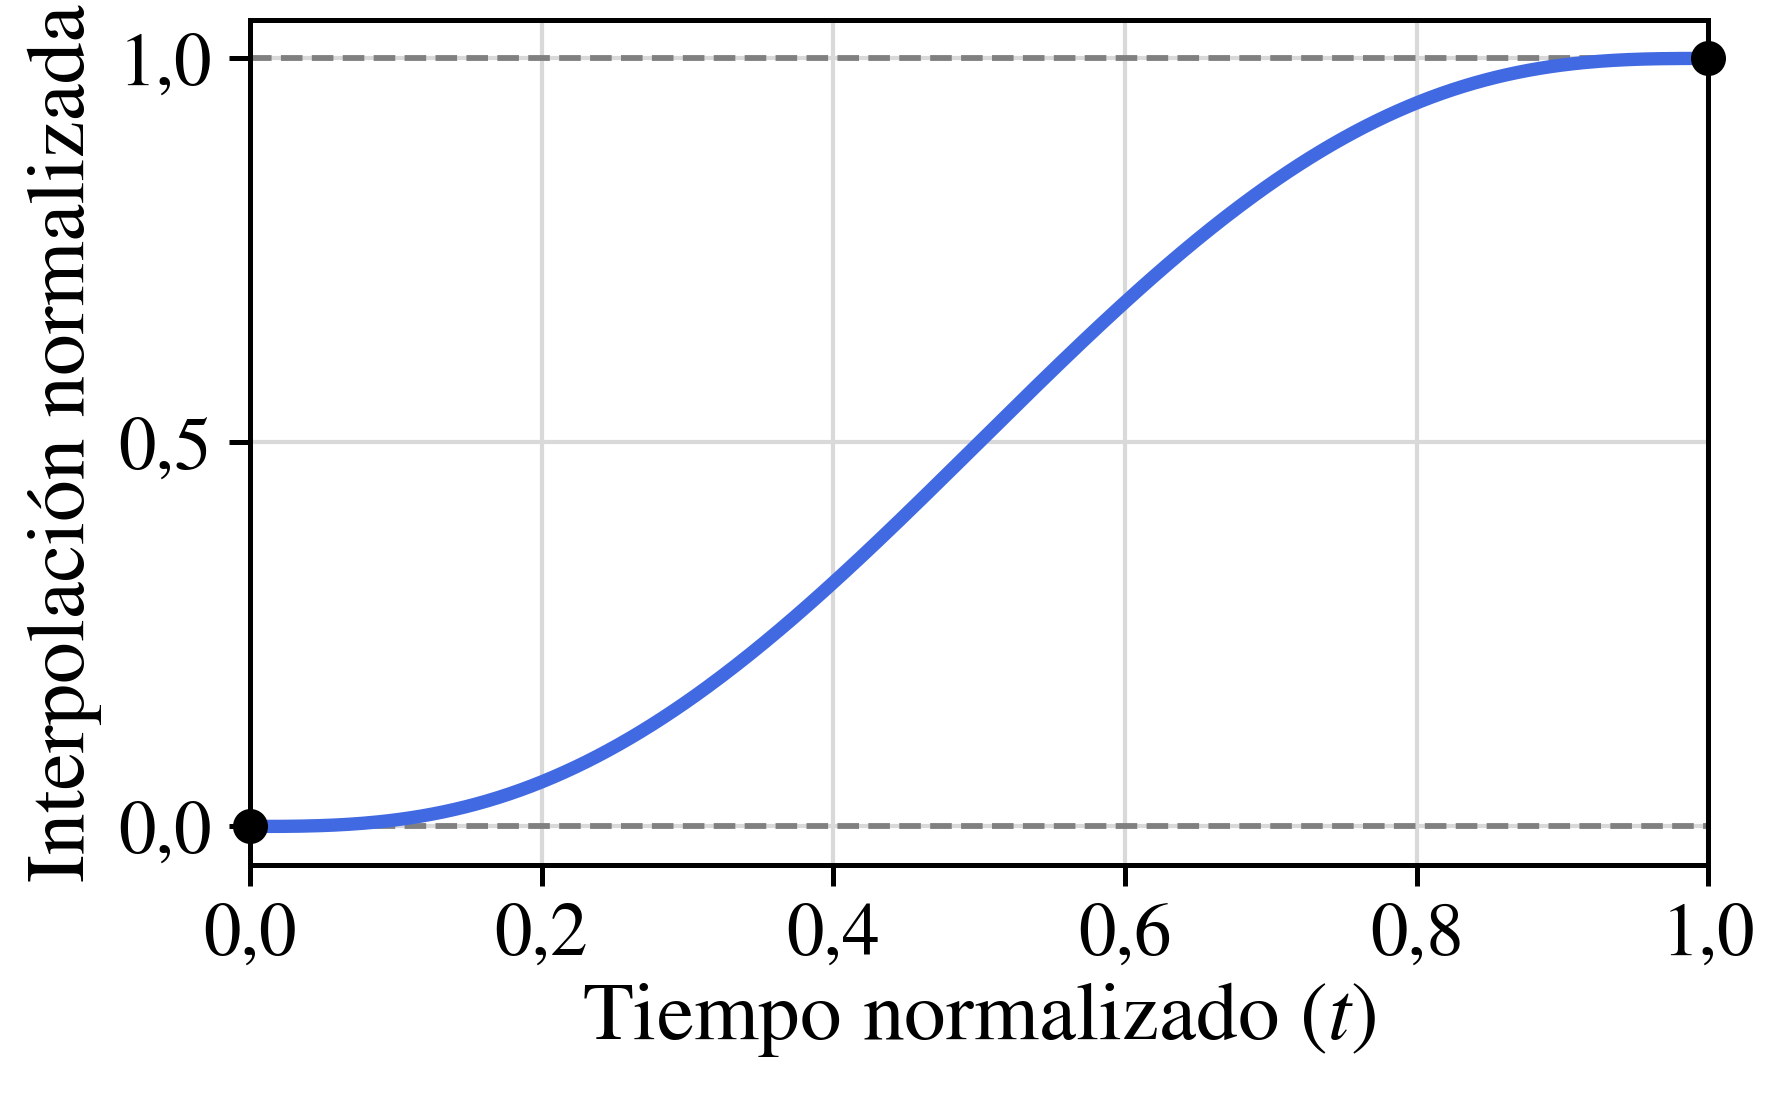
\includegraphics[width=\linewidth]{capitulos/cap2/figuras/quintic_pos.png}

    \vspace{0.1em}
    {\footnotesize (a) $S(t)=6t^5-15t^4+10t^3$.}
\end{minipage}
\hfill
\begin{minipage}[t]{0.47\textwidth}
    \centering
    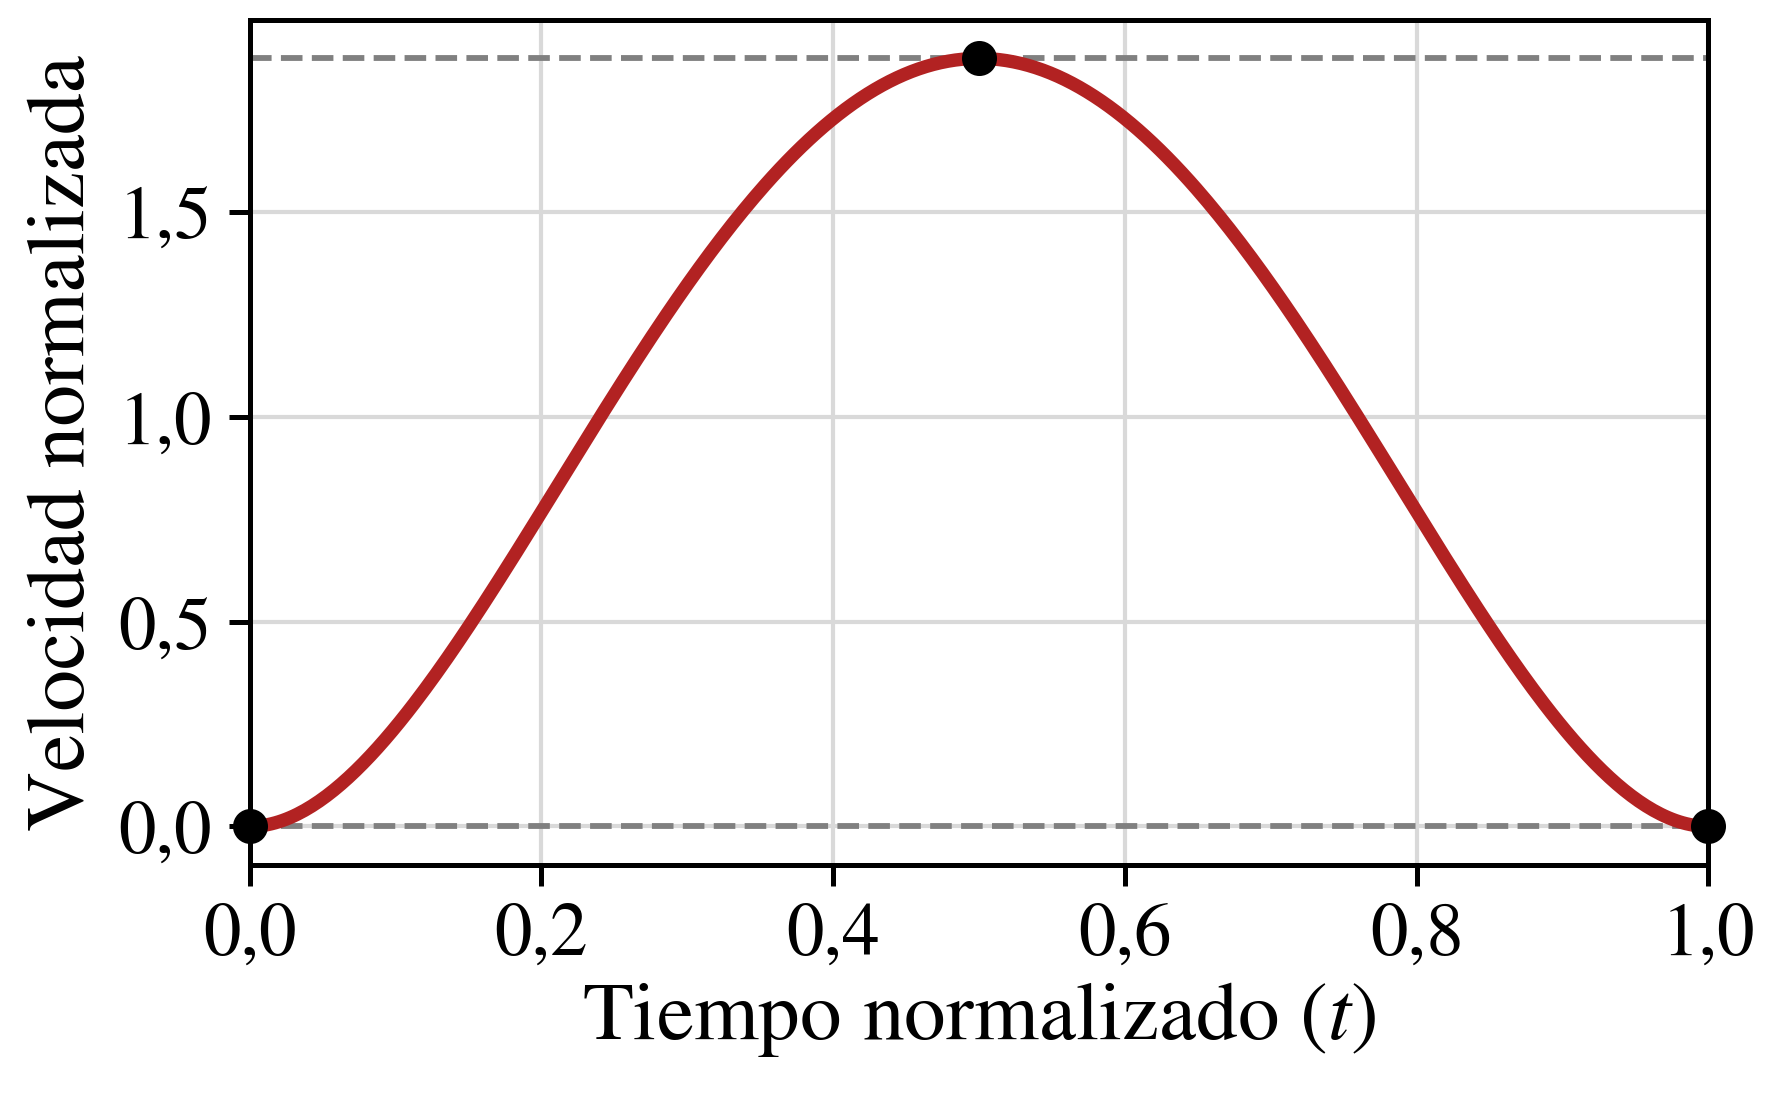
\includegraphics[width=\linewidth]{capitulos/cap2/figuras/quintic_vel.png}

    \vspace{0.1em}
    {\footnotesize (b) $\frac{d\,S}{dt}=30t^2(1-t)^2$.}
\end{minipage}

\vspace{0.35em}

\begin{center}
    \begin{minipage}[t]{0.47\textwidth}
        \centering
        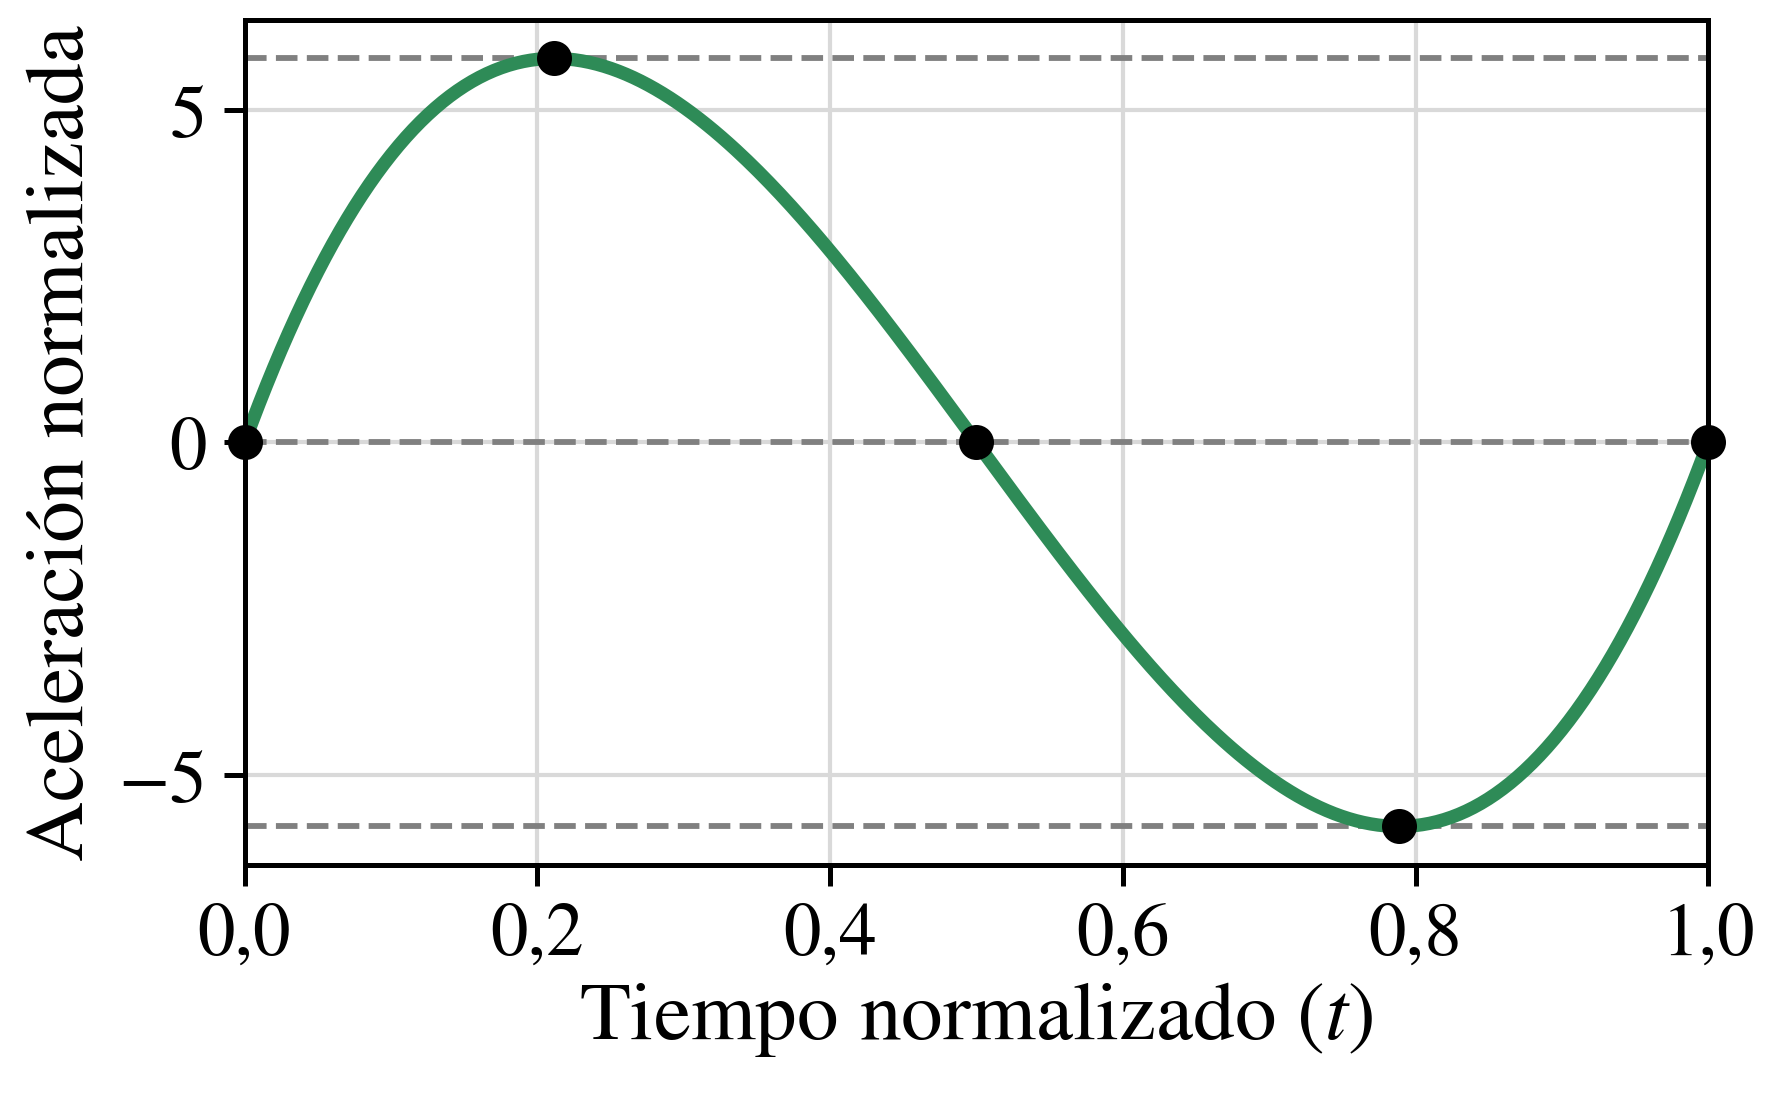
\includegraphics[width=\linewidth]{capitulos/cap2/figuras/quintic_acc.png}

        \vspace{0.1em}
        {\footnotesize (c) $\frac{d^2S}{dt^2}=60t(2t^2-3t+1)$.}
    \end{minipage}
\end{center}

\vspace{0.15em}
\begin{center}
    \captionsetup{type=figure,skip=2pt,justification=centering}
    \captionof{figure}[Perfil quíntico de suavizado]{Perfil quíntico de suavizado: evolución de la posición, la velocidad y la aceleración durante la transición de postura.}
    \label{fig:quintic_profiles}
    \par{\footnotesize Fuente: Elaboración propia mediante
    MATLAB~\cite{matlab}.}
\end{center}
